\chapter{灵长类动物前额叶皮层的进化} \label{chap:chap2}

\section{概述}
前额叶皮层(后文简称PF)的进化经历了不同的阶段。早期哺乳动物经历了一次进化,产生了所有哺乳动物共有的PF颗粒状前额区域。这些区域的产生能根据预测结果改善行动(第3章)和对象(第4章)之间的觅食选择。
早期灵长类动物经历了另一个进化,形成了第一个颗粒状的PF区域。
原本这些动物的仅在夜间生活于细小的树枝上,它们在那里寻找、选择和获取食物,用一种需要头部和一只手协调运作的方法进食。
他们进化后的PF区域有助于根据当前的生物需求和特定的习惯(第4章)来选择食物,以及在杂乱的环境中保持对食物的注意力(第5章)。
后来,在类人猿灵长类动物的进化过程中,随着这些物种及其大脑体积的增加,出现了额外的颗粒状 PF 区域。
它们依靠最新进化的灵长类中央凹和改进的色觉在白天觅食。 因此,可以比它们的祖先更好地处理时空事件的顺序(第6章)并对资源的迹象进行检测(第7章)。
因为丰富的资源分散在类人猿的园区范围内,它们面临着严峻的资源波动、捕食和竞争问题。
他们的新 PF 区域使他们能够通过使用单一事件来选择觅食目标(第8章)来减少风险和非生产性觅食选择的数量。

\section{介绍}
本章探讨了颗粒状前额皮层在早期灵长类动物中首次出现的结果,以及仅灵长类动物拥有这种皮层的事实(Preuss 2007a)。

由于其名称,一些神经科学家认为关于颗粒状前额皮层的进化历史仅取决于生物的细胞结构。考虑到这一主张的重要性,有人可能会争辩说这是一个薄弱的支撑。幸运的是,许多其他特征支持了“颗粒状前额皮层在灵长类动物中的进化”这一观点。接下来,我们将列出其中的四个特征:皮层区域之间的空间布局、颗粒状前额皮层向纹状体的投射模式、感觉输入的分布、以及通过电刺激皮层引起的自主神经反应。

图2.1展示了我们对人类、猕猴和老鼠这三个物种颗粒状前额皮层的同源性的看法,这主要归功于Preuss和Goldman-Rakic(1991a)的开创性工作。同源性指的是由于共同祖先的遗传而在相关物种中出现的类似区域。该图以浅灰色显示了仅在灵长类动物中进化出来的颗粒状前额皮层。这些颗粒状区域同样出现在人类和猕猴的大脑中,但不出现在老鼠的大脑中。老鼠只有无颗粒状前额皮层区域,该图为三个物种均以深灰色表示。我们选择这三个物种,是因为我们对前额皮层的大部分知识都基于对它们的大脑的研究。

\begin{figure}[!htb]
	\centering
	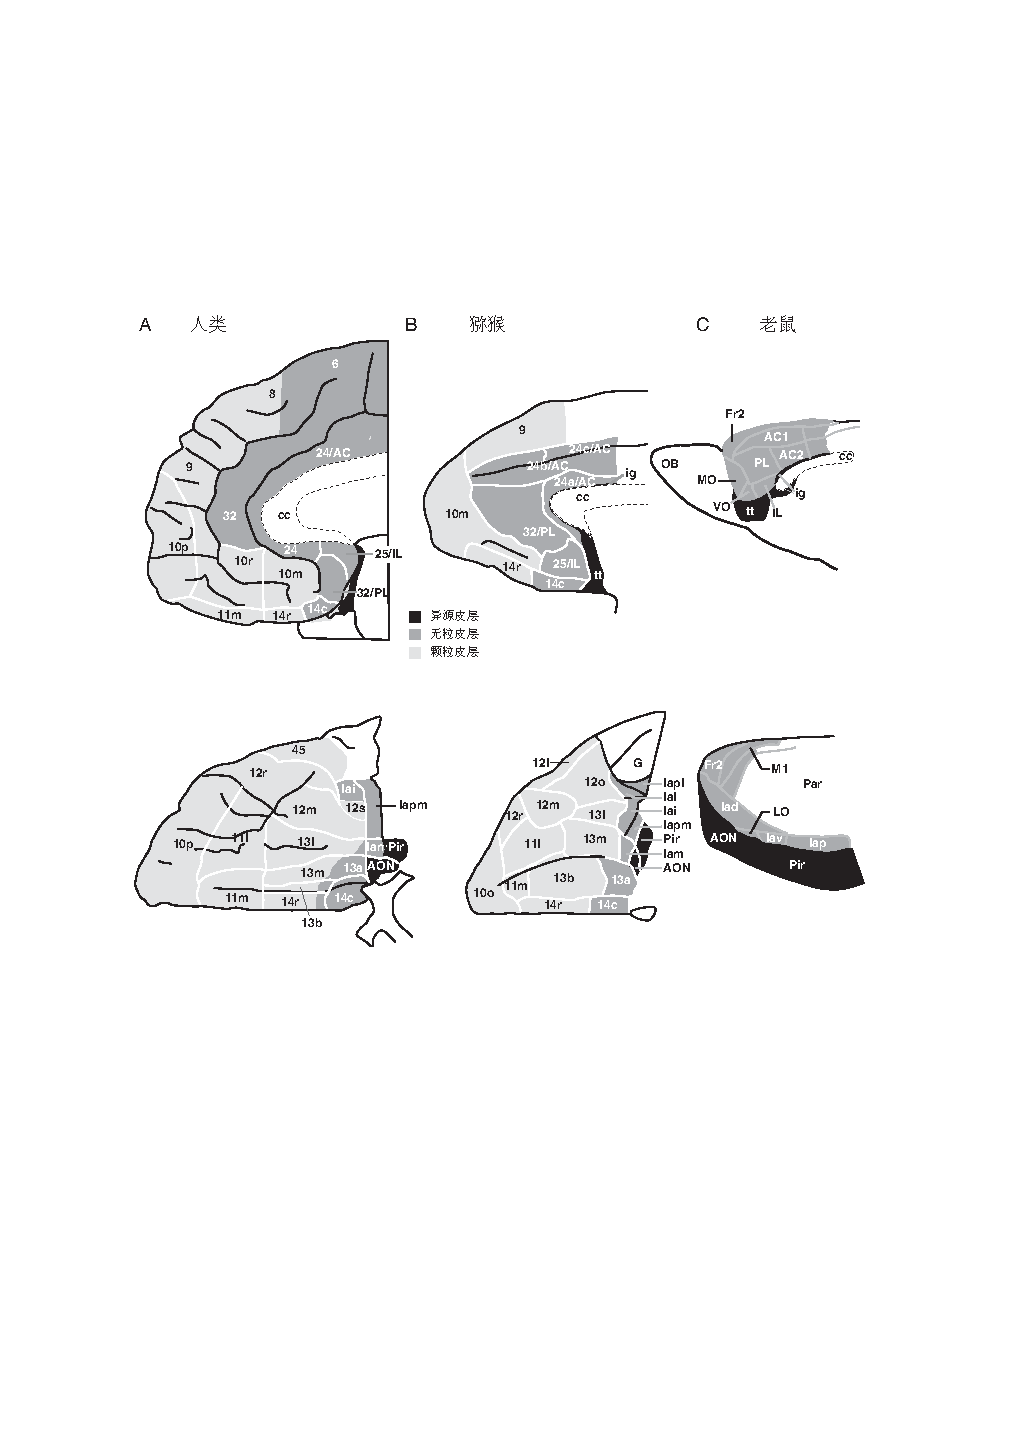
\includegraphics[width=0.8\linewidth]{image_pfc/Fig_2_1}
	\caption*{图2.1(A)人类前额皮层的内侧(上)和眶上区(下)(Ongur等人,2003)。 (B)猕猴前额皮层的内侧(上)和眶上区(下)(Carmichael\&Price,1994)。 (C)老鼠前额皮层的内侧(上)和侧面(下)(Palomero-Gallagher\&Zilles,2004)。在所有图中,向左为前端。上行:所有图中背面向上。下行:(A)和(B)中,侧面向上;在(C)中,背面向上。不按比例。缩写:AC,前扣带皮层;AON,前嗅“核”;cc,胼胝体;Fr2,第二额区;la,不含颗粒的岛叶皮层;ig,灰脑层;IL,下极叶皮层;LO,外侧眶上皮层;MO,内侧眶上皮层;OB,嗅球;Pir,锥体(嗅觉)皮层;PL,前扣带区;tt,盖带;VO,腹侧眶上皮层。区域细分标记为尾部(c);下(i);侧面(l),内侧(m);眶上(o),后部或极端(p),前端(r),或按任意标记(a,b)。 (A)改编自Ongur D. Ferry AT,Price JL。《人类眶上和内侧前额皮层的建筑分区》,《比较神经解剖学杂志》460:425-49,2003,经John Wiley和Sons许可使用。 (B)改编自Carmichael ST,Price JL.《猕猴颅内和眶上前额皮层的建筑分区》,《比较神经解剖学杂志》346:366-402,1994,经John Wiley和Sons许可使用。 (C)改编自Palomero-Gallagher N,Zilles K.《老鼠神经系统》中的异皮层.ed.G Paxinos,pp.729-57.圣迭戈,加利福尼亚州:爱尔斯维尔学术出版社。}
\end{figure}

非颗粒性前额叶皮层区域包括下肢内侧皮层、前扣带皮层、无颗粒的岛叶皮层、无颗粒的眶上皮层和前扣带回。在不同物种中,这些区域往往有不同的名称。例如,啮齿动物的下肢内侧皮层与灵长类动物的25区大致相对应,von Bonin和Bailey将其称为FL区(图1.1)。

众所周知,许多神经科学家认为老鼠拥有与灵长类动物相同的前额叶皮层。并且他们坚持认为,老鼠具有模拟灵长类动物前额叶皮层的微型复制品,或者可以将其所有属性混合在他们的小型无颗粒区域中(Kolb 2007;Seamans等人2008;Schoenbaum等人2009)。虽然我们对此持有不同的观点,但有一个命题应该得到普遍接受:在进化历史的某个时刻,我们的某些祖先缺乏颗粒性前额叶皮层。然而,现在我们不再缺失它。鉴于这个历史事实,询问颗粒性前额叶皮层带来了什么优势似乎是合理的。

尽管不是每个人都同意图2.1所描绘的同源性,但没有人严肃地质疑现代啮齿动物的大脑缺乏颗粒状前额叶皮层这一事实。对于其他哺乳动物,有一点存在争议:有人认为狗(Rajkowska\&Kosmal 1988)和猫(Rose\&Woolsey 1948)具有颗粒状前额叶皮层区域。但当我们亲自检查组织学材料中,狗和猫所谓的颗粒状区域时,它们看起来很像猕猴和啮齿动物的无颗粒区域。

正如第1章所述,这种争议可能是由于观察者缺乏成体系的知识方法所致。当Mackey和Petrides(2010年)在猕猴和人脑中观察到这个问题时,他们发现一些传统上被归类为无颗粒额叶区域的区域实际上在第4层细胞体密度上,与最尾端的区域相比有略微的增加。也就是说,这些区域具有较弱的非颗粒质细胞结构,而不是完全的无颗粒结构。在食肉动物和其他非灵长类哺乳动物中发现颗粒状PF皮层的报告,反映了这种属性。神经解剖学家们都认为,细胞从额叶轨道和内侧表面向头部移动时,第4层的厚度会持续增加。因此,无颗粒皮质是否在第4层完全消失并不重要。我们可以将第4层密度低于给定阈值的区域视为足够无颗粒这一标准,用于我们之后的研究中(如图2.2所示)。

尽管老鼠缺乏细颗粒前额皮层,但一些神经科学家仍认为,老鼠前额皮质的中部与灵长类动物的中侧颗粒前额皮层(区域46)同源(Kolb 2007; Seamans等人,2008),尽管后者的是一个颗粒区域(也称为背外侧或周主前额皮层)。同样,还有一些人认为,老鼠前额皮质的侧部与灵长类动物的整个眶前颞皮质同源,包括其颗粒部分(Kolb 2007; Schoenbaum等人,2009)。该论点基于解剖学、生理学和神经化学的相似性以及基于声称在老鼠和猕猴中的损伤效应的相似性。

\begin{figure}[!htb]
	\centering
	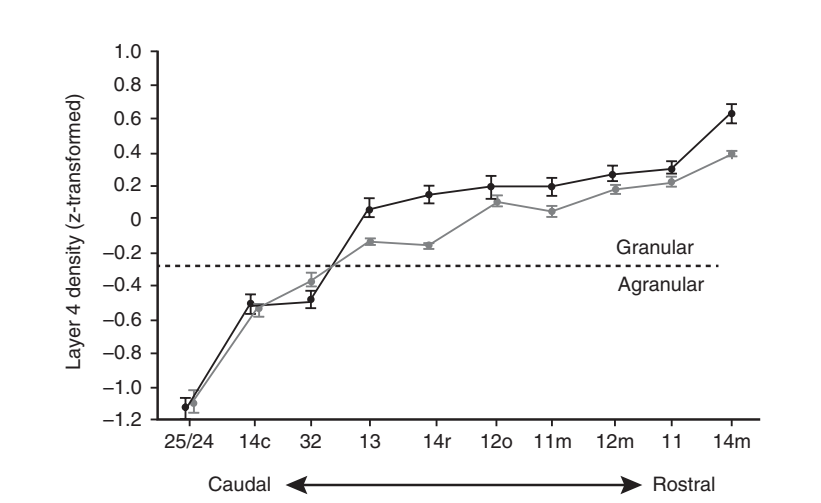
\includegraphics[width=0.8\linewidth]{image_pfc/Fig_2_2}
	\caption*{图2.2 显示了大脑额叶区域从尾向头发展的过程中,第4细胞层的归一化密度在猕猴(黑线)和人类(灰线)中的变化。误差条:SEM。该图由 Mackey S、Petrides M. 在《欧洲神经科学杂志》2010年32期(1940-1950页)中发表,经John Wiley 和 Sons出版社许可后再版。该图表明人类和猕猴大脑的腹内侧和侧壁眶前额皮质中具有可比较的成系统的区域。}
\end{figure}

然而,人们不能仅仅依据常被引用的相似性就推断其同源性。正如 Preuss(1995)所解释的那样,人们需要对特征进行诊断,即区分一组皮层区域和其他区域的特征。就像老鼠的非颗粒状前额皮质与猕猴的颗粒状前额皮质区域具有许多相似之处,例如编码估值的细胞。但是,这三个区域——老鼠的非颗粒状前额皮质以及猕猴的非颗粒状和颗粒状前额皮质——都具有与上述细胞同样的特性,其他皮层区域也是如此。因此,它们无法帮助我们理解前额皮层皮质的进化或建立其区域之间的同源性。例如,老鼠的非颗粒状区域的特性与灵长类动物的颗粒状前额皮质相似,但它们也与灵长类动物的非颗粒状前额皮质相似,那么这些特性就与动物的同源性无关。

有人声称,颗粒质前额皮层与丘脑中背核(MD)的联系是其诊断性特征(Rose\&Woolsey,1948年;Akert,1964年;Uylings等人,2003年)。但是,MD核向实际上覆盖了额叶的几乎所有区域,包括颗粒质和非颗粒质区域。因此,与MD核的连接不能作为诊断性特征,故它们对于同源性的问题几乎没有影响或很少有影响。

曾经有一段时间,人们认为多巴胺能输入是颗粒状前额皮质的特征(Divac等,1978;Porrino\&Goldman-Rakic,1982)。但是这些输入也终止于PF皮质的非颗粒状部分和运动前区,以及额叶以外大部分皮质。事实上,在灵长类动物中,多巴胺输入到运动前皮质和后枕叶皮质的强度比大多数颗粒状前额皮质都要强(Gaspar等人,1992;Williams\&Goldman-Rakic,1998)。因此,多巴胺输入不能帮助我们跨物种识别PF皮质。

最终,损伤结果得到了进一步的研究,例如对于延迟反应任务的研究结果。老鼠的前额内皮层损伤会导致该任务的障碍(Kolb等人,1974年),类似地,猕猴颗粒质前额皮层的损伤也会导致该任务的障碍(Goldman等人,1971年)。但是,前扣带回皮层的损伤也会导致猕猴在该任务上出现障碍(Meunier等人,1997年)。因此,该特征并非是诊断性的。我们将在第10章中更详细地讨论这个问题,老鼠和猕猴的障碍虽然表面上相似,但在重要的方面存在差异。

值得注意的是,我们并不是说灵长类动物拥有前额皮层而其他哺乳动物没有。我们认为非灵长类哺乳动物也有一些可以合理称之为前额皮层的区域。第3章和第4章将这些非颗粒质区域纳入了内侧和眶前颞皮层。但我们不赞同非灵长类哺乳动物具有类似于灵长类前额皮层的微型复制品或混合体的观点。非灵长类哺乳动物缺乏灵长类动物的颗粒质前额皮层以及执行其基本功能的任何区域。因为忽略了这些概念,文献中存在很多将非同源区域的结果混合在一起的实例,例如,引用灵长类动物的中侧前额皮层(46区)的研究结果来支持与啮齿动物的前额内皮层相关的某些结论。但其实这不是最好的方式。

我们对同源性的结论不应该引起太多争议。以视觉皮层为例,所有灵长类动物都共享10-20个视觉区域,其中有些物种甚至拥有更多的视觉区域(Kaas,2006年)。举个例子,一个被称为MT或V5的区域在视网膜中央凹有精细的专门分化功能,用于分析视觉运动。但老鼠的视觉区域少得多(Rosa\&Krubitzer,1999年;Lyon,2007年),不可能复制灵长类动物10-20个视觉区域的所有功能,并且它们缺乏中央凹。另外,在缺乏中央凹的物种中进行视网膜中央凹的微观分析是不太可能的。

再以另一个例子为例,考虑到蝙蝠听觉皮层的回声定位功能。这些动物使用类似声纳的系统来检测它们与猎物的距离和猎物本身的速度。蝙蝠的听觉皮层有许多专门区域来处理与回声定位相关的声学信号,包括分析调频声音、多普勒频移等等(Suga等人,1997年;Fitzpatrick,1998年)。但如果老鼠的听觉皮层中的一些细胞也对类似的声音作出反应,这并不意味着它们执行与蝙蝠听觉细胞相同的功能。事实上,想象它们这样做是很奇怪的,因为老鼠不会用回声定位来追踪它们的食物。同样,认为老鼠的少数听觉区域具有与回声定位蝙蝠的大量专门区域相同的所有功能和属性是缺乏可信度的。

很少有神经科学家质疑这样一个想法:与老鼠共同祖先相比,声呐定位蝙蝠拥有新的听觉区域,而灵长类动物拥有新的视觉区域,以适应其在视觉敏锐度和色彩视觉方面的需求。同时,这些新区域支持新的功能,如对凹视动作或回声定位的分析,这一观点已经被广泛接受。因此,令人惊讶的是,同样的神经科学家们往往对这样一个想法犹豫不决:灵长类动物拥有新的前额区域,并且这些区域具有新的功能。

问题的一部分来自于使用“新”的词来描述区域或功能。有人提出,新的区域通过复制和随后的分化出现(Krubitzer\&Huffman 2000)。如果是这样的话,那么合理的假设是,某些新区域的分化程度比其他区域低;当它们在许多哺乳动物中出现时,我们可以将更保守的区域识别为同源的。然而,在这样做时,我们需要认识到大多数进化所产生的变化都涉及到同源结构的修改,因此在物种之间具有绝对等价是不现实的。

相较于这些相对保守的区域,其他的复制产物则更加具有差异化,因此应该被称为新的区域。随着差异化的产生,它们开始执行新的功能,从而提供了优于其祖先状态的优势。然而,当这些新区域进化时,它们会与附近的区域共享属性,并且通常会与它们有轴突连接。因此,虽然PF皮层的颗粒层和无颗粒层部分具有许多共同特征。但是我们不应该基于此得出它们是同源或类似的结论。颗粒状的PF皮层专门在灵长类动物中进化而来,并发展为支持灵长类动物具有特别能力的区域。

\section{原猴亚目前额叶皮层}
灵长类动物 PF 皮层进化的最有力证据来自对原猴亚目的研究。鉴于这一证据的重要性,我们将详细地回顾它。然而,读者可以从本节末尾的摘要中了解该论点的要点。

讨论中必要地使用了一些可能不是所有神经科学家都熟悉的术语,因此表2.1列出了这些术语以便参考。主要的灵长类动物群组包括原猴亚目、原猴类、类人猿亚目和类人猿。在进化过程中,灵长类动物分裂成原猴类(湿鼻)(lemurs, lorises), 和丛林婴猴,构成了大多数称为原猴亚目的灵长类动物)和类人猿亚目(干鼻)(包括狐猴,人猿和类人猿)。类人猿亚目包括所有新大陆猴(Platyrrhines),以及旧大陆猴、大猩猩和人类(统称为狭鼻猿)。

\begin{table}[htbp]
	\newcommand{\tabincell}[2]{\begin{tabular}{@{}#1@{}}#2\end{tabular}} %换行指令
	\centering
	\caption{本章中使用的生物学术语}
	\renewcommand\arraystretch{1.5}	%设置表格内行间距
	\begin{tabular}{ll}
		\toprule
		术语 & 含义 \\
		\midrule
		进化 & 与祖先状态不同,具有差异化的  \\
		埃及古猿 & 一种已灭绝的类人猿,接近早期的狭鼻类动物  \\
		类人猿 & 猕猴、猿类和人类  \\
		食果猴 & 一个已经灭绝的古老哺乳动物类群  \\
		智利猴 & 一个灭绝的类人猿,接近于最早的阔鼻猴  \\
		狭鼻猿& 旧大陆灵长类动物(旧大陆猴、类人猿和人类),从阔鼻猿中分化出来  \\
		类人猿亚目& 眼镜猴与类人猿;从原猴类中分化出来  \\
		同源性& 从共同祖先继承而来的相似性,与由平行或趋同进化引起的相似性形成对比  \\
		旧大陆猴& \tabincell{c}{一组狭鼻猴类灵长目动物,包括猕猴、狒狒、长尾黑颚猴(绿猴)、\\白眉猴、长尾猴、山魈猴和红尾猴}  \\
		%内容换行
		副猿& 已灭绝的类人猿,接近于第一个类人猿,也被称为Simonsius  \\
		阔鼻猴& 新大陆猴,包括鬃狮猴、松鼠猴、枭猴和卷尾猴;从狭鼻猿中分化出来  \\
		更猴形类群& 已经灭绝的哺乳动物,可能是早期灵长类或早期灵长类的近亲,包括食果猴  \\
		原始的& 类似于祖先的情况  \\
		原猴亚目& 原猴类灵长类动物和猴鼠目动物; 不构成一个天然类群  \\
		原猴类& 大多数原猴类灵长类动物,包括狐猴、懒猴和丛林婴猴;从类人猿中分化出来  \\
		\bottomrule
	\end{tabular}%
\end{table}%

接下来,我们假设现代灵长类动物和类人猿共有的特征可能存在于它们最后的共同祖先身上。由于那个祖先是早期的灵长类动物,因此我们认为这些特征也是早期灵长类动物的特征。我们还假设类人猿具有但灵长类动物没有的特征可能是在类人猿中进化出来的。像之前一样,在形成分支后,独立进化也在继续进行,因此灵长类动物可能具有类人猿所缺乏的适应性。

Preuss和Goldman-Rakic(1991a)认为,和几个其他颗粒状前额皮层区域一样,灵长类动物的皮层缺乏中侧PF皮层(区域46)的同源区。相反,他们确定了尾部PF皮层(区域8)和眶上PF皮层的颗粒状部分的同源区。Preuss和Goldman-Rakic用各种论证支持了他们的结论,其中包括比较丛林婴猴和恒河猴的共同之处(Preuss\&Goldman-Rakic 1991b)。他们还考虑了其他人在狐猴(另一种原猴类灵长类动物)上所做的工作。然而,他们大部分证据来自于对丛林婴猴和恒河猴前额皮层结构的研究。最近一项研究确认了他们所分析的大部分内容(Wong\&Kaas 2010)。

\subsection{皮质结构}
图2.3显示了Preuss和Goldman-Rakic为丛林婴猴额叶皮层绘制的图。在本节中,我们将对其进行详细的介绍与分析,以供对解剖学细节感兴趣的读者参考。

首先,Preuss和Goldman-Rakic确定了运动前皮层的不含颗粒的区域(区域6)。在紧贴区域6的前额叶表面皮层上,包括一个独特的区域,具有“非常厚、密”的第4层和髓鞘化的纤维束,这些纤维束从皮质下白质向第4层延伸,在那里分散到更浅的层中。

Preuss和Goldman-Rakic得出结论,这个被称为后颗粒区(GrP)的区域(图2.3)与猕猴和人类的8区同源。在该区域的进行电刺激会引发灵长类动物(Wu等人,2000)和猕猴(Bruce等人,1985)的眼动作,这一发现支持了GrP区域包括前额眼场(FEF)的结论。

\begin{figure}[!htb]
	\centering
	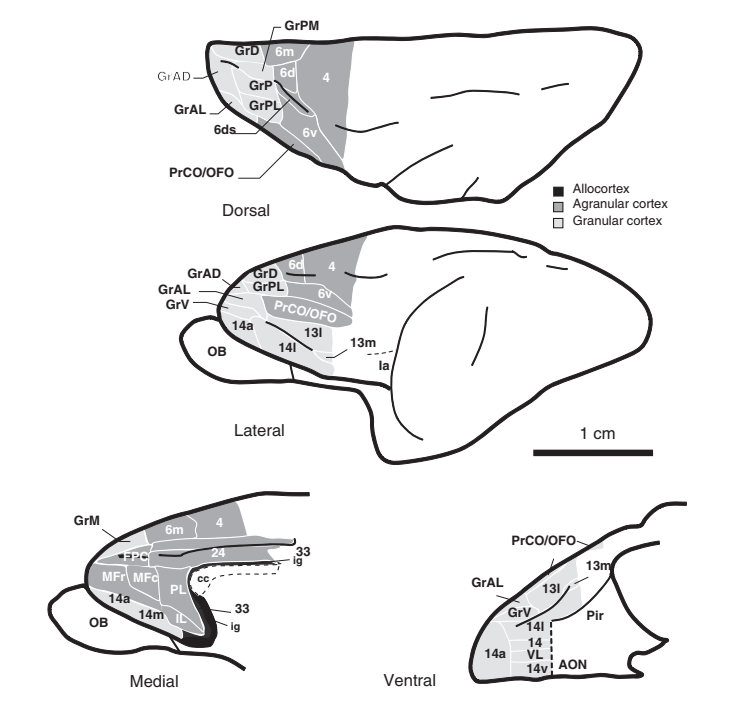
\includegraphics[width=0.8\linewidth]{image_pfc/Fig_2_3}
	\caption*{图2.3:灵长类动物额叶皮层的建构图。所有图中,前端朝左。从上到下依次为背侧视图:向内为上;侧面视图:背侧向上;内侧面视图:背侧向上;腹侧面视图:侧面向上。缩略语如图2.1所示,包括以下内容:Gr,颗粒区,分为前部(A),背部(D),侧部(L),中部(M),后部(P);PrCO/OFO,前中央卷叶区/眶前额叶卷叶区;6ds,背区域6的沟部分;FPC,额极回扣带区;MF,中央前额叶皮质;VL,腹侧区域。摘自Preuss TM,Goldman-Rakic PS。灵长类动物狨和人猿类动物猕猴的颗粒前额叶皮层及其周围区域的髓样和细胞样结构。《比较神经学杂志》310:429-74  1991,John Wiley and Sons,获准使用。}
\end{figure}

Preuss和Goldman-Rakic指出,区域GrP在内侧被后-中颗粒区(GrPM)包围,在外侧被后-侧颗粒区(GrPL)包围(见图2.3)。他们认为GrPM和GrPL分别对应于8Ad区和45区的一部分。这个结论并不仅仅是基于它们与GrP和6区的拓扑关系。Preuss和Goldman-Rakic还指出,在灵长类动物和恒河猴的内侧和外侧区域中,锥形细胞比GrP区域小,横向定向的髓鞘束比GrP区域更显著。根据类似的基础,他们得出结论,更内侧的区域称为背颗粒皮层(GrD)和内侧颗粒皮层(GrM)(见图2.3),分别与恒河猴的8B区的背部和内侧部分同源。

Preuss和Goldman-Rakic稍微不那么自信地指出,他们推测了灵长类动物的颗粒质PF皮层更向前部位的同源区,例如前背侧颗粒区(GrAD)。他们还考虑了两种可能性:一种是灵长类动物的GrAD与猕猴和人类的区域8Ad的前部同源。这个想法基于GrP仅与猕猴的区域8Ad的尾部同源,留下其前部“自由区域”成为GrAD的同源区。另一种可能性是,GrP可能是猕猴的区域8Ad的前部和尾部的组合同源区。在这种解释下,区域GrAD可能与猕猴大脑中的后外侧PF皮层(区域9/46)同源,或者由于其与后顶叶皮层之间的联系不强,与极端PF皮层同源(Preuss 2007a)。这个问题还没有解决,但重要的是,Preuss和Goldman-Rakic没有发现GrAD与中侧PF皮层(区域46)对应的证据,这个结论受到了区域GrAD与后顶叶皮层之间连接较弱的支持。

至于眶额叶皮质,Preuss和Goldman-Rakic建议,灵长类动物的腹侧颗粒区(GrV)可能对应于猕猴的11区(参见图1.2)。并且,总体而言,他们得出结论是灵长类动物具有与猕猴差不多数量的眶部亚区。

Preuss和Goldman-Rakic无法确定类似于GrAL的区域在狨猴脑中的同源区,因此他们认为这个区域是在类狨目和类灵猴目分化后在狨猴中演化出来的。

作为他们最重要的观点之一,Preuss和Goldman-Rakic指出,许多猕猴大部分PF区域的髓鞘比额叶皮层的要少,而且在灵长类动物的额叶皮层中似乎不存在这样的髓鞘较少的区域。一项最近的结构成像研究将这个论点扩展到黑猩猩和人类中(Glasser等人,2011)。除了一些基于连接性的论证之外,他们得出了这样的结论:除非灵长类动物中的灰瘤质区域与其他动物有所不同,否则包括9、12/47和46区域以及可能的10区域在内的这些髓鞘较少区域在灵长类动物演化中是在单鼻亚目分化后进化出来的,而现代的猕猴、大猩猩和人类通过继承拥有了它们。刚才提到的所有区域都具有灰质细胞形态学和少量的髓鞘,并且它们构成了现代人猿类,包括人类的大部分PF皮层。

\subsection{拓扑结构}
拓扑学术语指的是大脑皮层结构的空间排列方式,具体指皮层区域在二维皮层平面内的相对位置,可以想象将其展开以显示脑沟和脑回。例如,Preuss和Goldman-Rakic使用GrP与运动前皮质(区域6)之间的拓扑关系来确定它是短尾猴额叶眼区(FEF)的同源物。拓扑学术语在皮层进化的出版讨论中很少使用,但空间结构之间的证据一直是评估同源性最重要的特征之一。通常情况下,邻近结构为解释某些原本难以理解的结构提供了重要的指导,这是因为身体的基本模式在进化发育中是比较保守的特征之一。

前额皮层拓扑结构中一个特别重要的方面涉及它与异皮层的关系。如图2.1所示,一些前额区域直接相邻于黑色所示的异皮层。与大多数大脑皮层相比,异皮层仅有三个层次,其层次结构相对简单。典型的例子包括海马体和嗅叶皮层。

PF皮质的非颗粒部分靠近分配性皮层。例如,在啮齿类动物和灵长类动物中,无颗粒岛叶皮质毗邻嗅叶皮质和前嗅核。尽管前嗅核被称为“核”,但它是一种分配性皮质结构。其他非颗粒额叶区域,如前扣带皮质、下肢内侧皮质和前肢内侧皮质,毗邻更小、更不为人知的分配性皮层区域。虽然一些权威机构已经为靠近分配性皮层的皮层区域开发了复杂的名称,例如近分配皮层或前等皮层,但我们主要是基于比较的原因将它们全部视为新皮质的变体。

因此,非颗粒性前额皮质区域不仅可以通过其细胞结构进行识别,还可以通过它们与非皮层相邻来识别。相比之下,颗粒性前额皮质区域不与非皮层相邻,而是靠近非颗粒性前额皮质区域。因此,拓扑学和细胞结构都认为颗粒性前额皮质区域与非颗粒性前额皮质区域不同。需要注意的是,这种分析不包括运动皮层和前运动区,尽管它们也是非颗粒性的。

\subsection{皮质投射}
我们的论点也得到了某些皮质投射的支持。例如,在啮齿动物中,通常称为眶前额叶皮层或眶额皮层的区域向纹状体发送直接投射。仔细研究这个投射的细节提供了一些诊断特征,基于这样一个假设,即额叶皮层的同源部分向纹状体的同源部分投射。

在老鼠中,来自下肢内侧区和前扣带区的投射主要终止于伏隔核壳,这是腹侧纹状体的一部分(Brog等,1993; Reynolds\&Zahm,2005)。纹状体分为两部分,腹侧纹状体包括伏隔核以及其他一些结构,而背侧纹状体包括尾状核和腹侧核。猕猴的25区和32区也投射到伏隔核壳(Haber等,1995,2006; Ferry等,2000),这一特征支持它们与啮齿动物中被称为下肢内侧区和前扣带区的区域的同源性。

在猕猴中,颗粒状前额皮层区域根本不投射到任何地方的伏隔核,更不用说它的壳了,它们也不投射到任何其他的腹侧纹状体区域。相反,它们投射到背侧纹状体的一部分,具体来说是尾状核(Selemon \& Goldman-Rakic 1985)。因此,从详细的皮层-纹状体终止模式得出的结论与从细胞结构和拓扑学得出的结论一致。颗粒状前额皮层没有在老鼠中的同源物。

同样的规律也适用于眶前额叶皮层。在老鼠中,眶前额叶皮层投射到腹侧纹状体或其附近(Berendse等人,1992年)。在猕猴中,眶前额叶皮层的无颗粒部分(包括无颗粒岛叶区域)向这些纹状体部位发送大量的投射。但是,额叶皮层颗粒质部分投射到背侧纹状体。与半球外侧颗粒质PF区域一样,额叶表面的颗粒质区域主要投射到尾状核(Haber等人,1995年,2006年;Ferry等人,2000年;Öngür和Price,2000年)。

神经解剖学家描述了灵长类动物中新的前额叶皮层区域及其皮层纹理-尾纹突出部向腹侧移位的现象,将其称为“腹侧移位”(Schilman等人,2008年)。在老鼠中,非颗粒层的前额叶皮层投射于纹状体的背部和腹部之间。然而,在灵长类动物中,同源的非颗粒层的前额叶皮层的投射终止于纹状体的腹部三分之一位置。这种腹侧移位与新的前额叶皮层区域投射到更背部的纹状体区域是一致的。

我们在这里指出的现象,与那些认为啮齿动物的背内侧纹状体与灵长类动物的尾状核是同源的人存在分歧的主要原因是基于拓扑学(Balleine\&O'Doherty 2010)。在啮齿动物中,内囊并没有像在灵长类动物中那样将尾状核与壳核分开。这使得在背纹状体内进行同源性分配变得困难,这也是为什么Balleine和O'Doherty得出他们的结论的原因。然而,他们的同源性观点几乎没有任何来自比较神经解剖学的支持。灵长类动物的尾状核的一个小的腹部可能在啮齿动物中有同源物。然而,尾状核的头部以及向其投射的纹状前额皮质区域是在灵长类动物中进化形成的。

此外,Preuss(1995)指出,在灵长类动物中,相比于灰质PF区的皮质-上丘(superior colliculus)弱的皮质-上丘投射,灰质PF区对皮质-上丘的投射更为强烈。然而,我们不认为这是一个主要的论点。虽然它适用于灰质PF皮层的背侧、内侧、腹侧、极性和尾侧,但眶上PF区对皮质-上丘的投射并不显著(Leichnetz等人,1981)。

\subsection{感官输入}
额外的联系支持了我们的论点。在老鼠和猕猴中,无颗粒PF皮层的部分相对直接地接收嗅觉、味觉和内脏输入(Ray \& Price 1993),正如第4章更详细地讨论的那样。嗅觉输入来自梨状皮层;味觉和内脏感觉输入通过脑干和丘脑中继抵达无颗粒PF皮层。这些联系支持了灵长类和啮齿动物无颗粒轨道区域的同源性。轨道PF皮层的颗粒状部分缺乏这种特征,仅通过无颗粒额叶区间接地接收这些感觉输入。

\subsection{自主输出}
啮齿动物和灵长类的无粒质前额叶皮层与灵长类的颗粒状前额叶皮层还有其他不同之处。来自无粒质前额叶皮层的输出比颗粒状前额叶皮层更直接地影响自主神经系统。如图2.4所示,电刺激猕猴的最后部分的颞上回皮层,包括无粒质岛层,以及前扣带回皮层和下肢回皮层会引起自主反应(Kaada 1960)。这些反应包括呼吸速率的变化、血压的变化、脉率的变化、瞳孔扩张和毛发竖立。颗粒状前额叶皮层的刺激,包括颗粒状的部分,没有这样的效果(Kaada等人1949)。

\begin{figure}[!htb]
	\centering
	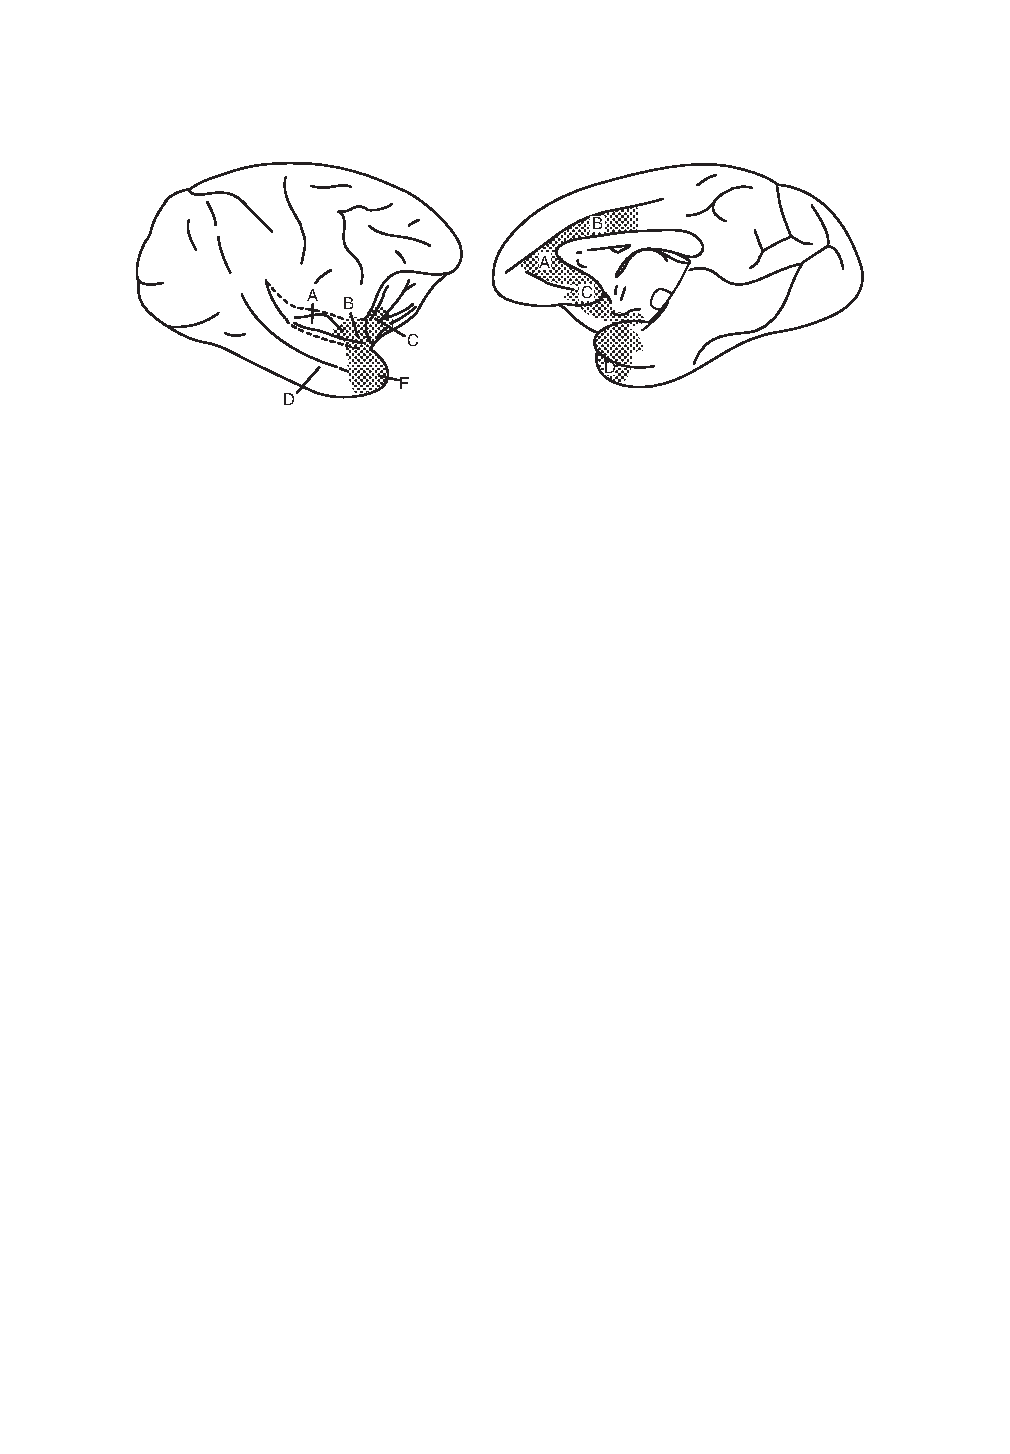
\includegraphics[width=0.8\linewidth]{image_pfc/Fig_2_4}
	\caption*{图2.4 展示了对猕猴大脑区域进行电刺激引发自主神经效应的区域(用点状线填充)。左图为侧面视图,右图为内侧视图。左图中电刺激区域包括:A,颗粒和非颗粒岛叶皮层(无效应);B,非颗粒岛叶皮层;C,尾侧(非颗粒)眶额皮层;D,颞下皮质(无效应);F,颞极皮层。右图中电刺激区域包括:A,前扣带皮质(见第三章);B,前扣带皮层;C,亚扣带、下肢带皮层;D,颞极皮层。注意,刺激非颗粒区域会产生自主神经效应,而刺激颗粒区域则没有(Kaada等人,1949年)。图表取自《Journal of  Neurophysiology》杂志,版权归美国生理学会所有,已获得授权使用。}
\end{figure}

沃克(1940年)的额叶皮层地图并没有意识到13区和14区具有颗粒和无颗粒部分,但其他人已经注意到眶前额皮层后部具有无颗粒的细胞结构(Carmichael\&Price 1994年)。图2.1说明了14c区和13a区的这种特性,Mackey和Petrides(2010年)最近通过定量细胞结构分析对此进行了确认(图2.2)。Carmichael和Price(1994年)将无颗粒岛叶皮层包括在PF区的眶组中,这进一步加强了基本观点。

如果其他哺乳动物的无颗粒PF区与灵长类动物的无颗粒PF皮层同源,那么对这些区域的电刺激应该产生自主神经效应。正如预测的那样,这个特性已经在老鼠、兔子、猫、狗、多种猕猴和人类中得到证实。例如,刺激内侧PF皮层会在兔子(Powell\&Ginsberg 2005)和老鼠(Scopinho等人2009)中引起心动过缓。此外,兔子(Powell等人1997)和老鼠(Frysztak\&Neafsey 1994)无颗粒PF皮层的损伤会破坏预测生理应激物的刺激对自主反应的调节。

\subsection{小结}
颗粒状前额叶皮层和无颗粒前额叶皮层的区别不仅由皮层细胞结构和髓鞘结构支持,还由区域之间的拓扑关系、皮质纹状体连接的模式、感觉输入和自主输出的模式支持。因此,通过比较灵长类动物与其他哺乳动物,我们可以得出以下结论:\par
1.非灵长类哺乳动物缺乏灵长类动物颗粒状前额皮层的同源结构;\par
2.灵长类动物和其他哺乳动物具有几个同源的无粒状前额皮层区域:下肢前区、前扣带回、前扣带皮层、无粒状眶区和无粒状岛叶皮层;\par
3.这些无颗粒前额皮层区域可能是从最早的哺乳动物所演化出来的,因为迄今为止检查过的所有哺乳动物都有这些区域的同源结构,而在非哺乳类脊椎动物中没有发现同源结构。

\begin{figure}[!htb]
	\centering
	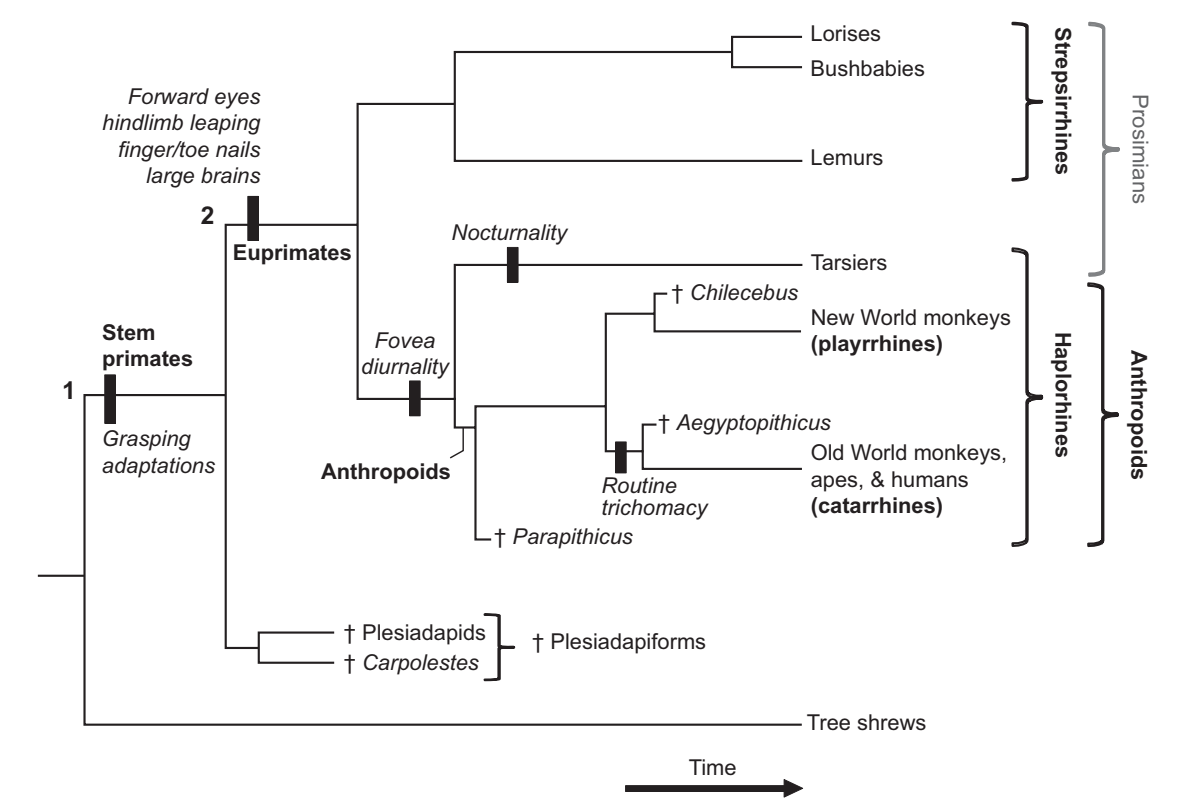
\includegraphics[width=0.8\linewidth]{image_pfc/Fig_2_5}
	\caption*{图2.5:所选现代和灭绝灵长类动物之间的进化关系。黑色条纹表示某些分支线路的创新,每个条纹旁标有斜体字注明创新特征。右侧方括号中的组,黑色表示自然群(类群),灰色表示其他(近源)群。†表示已灭绝的群体。1和2表示关于灵长类动物最近共同祖先的不同观点。}
\end{figure}

\begin{figure}[!htb]
	\centering
	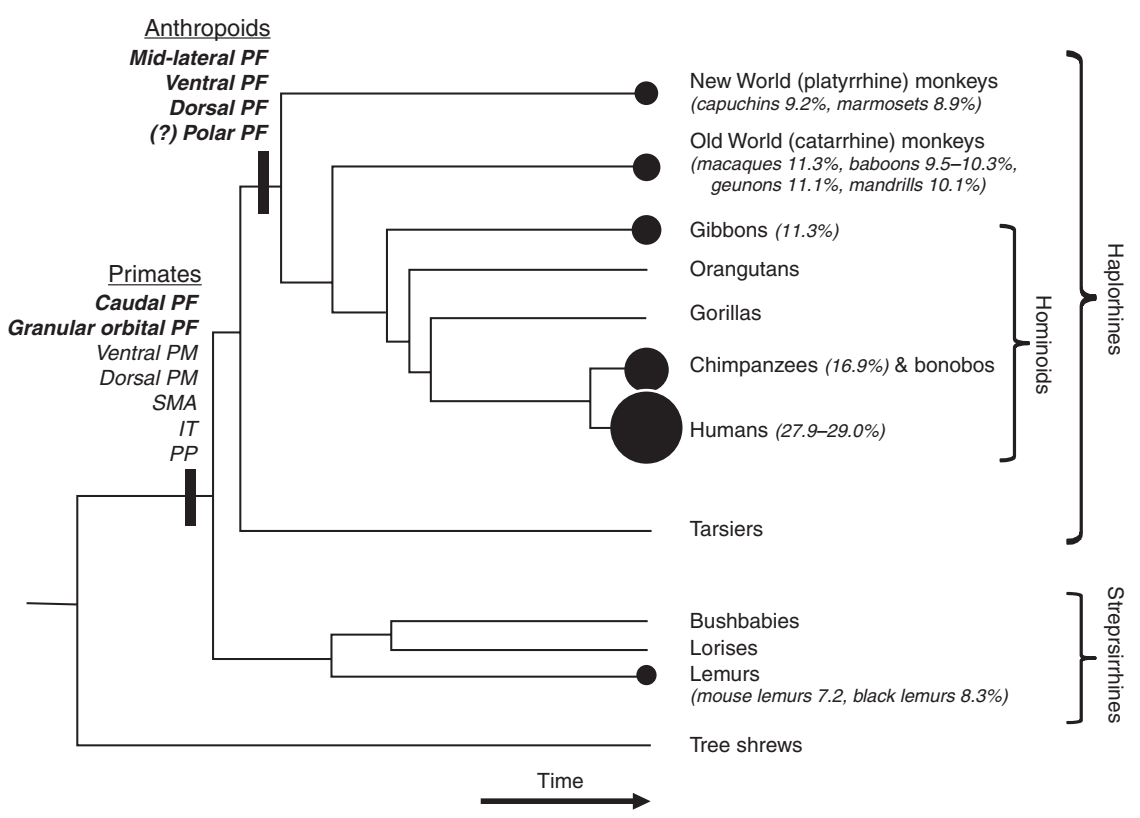
\includegraphics[width=0.8\linewidth]{image_pfc/Fig_2_6}
	\caption*{图2.6 选定的灵长类物种和树鼩之间的进化关系。缩写:IT,颞下皮质;PF,前额叶皮质;PM,前运动皮质;PP,后顶叶皮质;SMA,辅助运动区。每个末端圆圈的直径与包括颗粒前额叶皮质的皮质比例成比例,所选物种的百分比标在每个圆圈右侧。格式与图2.5相同,只是时间尺度是线性的。}
\end{figure}

通过比较一个代表性的猴形目灵长类动物(如猕猴)与一个代表性的原猴亚目动物(如灰背树鼩)的大脑,我们可以得出第二组结论。图2.5展示了这些灵长类动物的关系,以及随着某些谱系的出现而出现的特征,这些特征可以在黑色条形上方或下方找到。图2.6指出了早期灵长类和猴形目动物中进化出来的一些皮层区域。\par
1.原猴类动物缺乏类人灵长类动物中存在的几个区域的同源,包括中侧前额叶皮质(区域46),背内侧前额叶皮质(区域9)和腹侧前额叶皮质(区域12/47)。我们认为后外侧皮质(区域9/46)和极前额皮质(区域10)也属于这一类别,尽管这些点的证据仍不够全面;\par
2.这些新区域是在原猴类和类人猿亚目分裂之后进化出来的,可能是在人猿类中进化出来的,后文我们会解释;\par
3.原猴类和类人猿共享两组区域。第一组包括所有哺乳动物都有的无粒界额叶皮层区域;第二组则对应于早期灵长类动物进化出来的有粒界额叶皮层区域,其中包括前额眼场(FEF)和颅后无粒界额叶皮层(区域8)的其他部分,以及眶上的有粒界额叶皮层部分。

\begin{table}[htbp]
	\centering
	\caption{在哺乳动物、原猴类和类人猿中具有同源 (+) 或可能具有同源 (?) 的皮层区域}
	\setlength{\tabcolsep}{8mm}	
	\renewcommand\arraystretch{1.5}	
	\begin{tabular}{lllll}
		\toprule
		区域 & 来源 & 哺乳动物 & 原猴类 & 类人猿 \\
		\midrule
		背内侧皮层 & a & & &+  \\
		中侧皮层 & a & & &+  \\
		腹侧皮层 & a & & &+  \\
		尾部主要运动皮层 & b,c & & &+  \\
		后外侧皮层 & a & &? &+  \\
		极前额皮层&  a & &? &+  \\
		尾部前额皮层&  a & &+ &+  \\
		前额眼区& a,c & &+ &+  \\
		颗粒状眶前额皮层& a & &+ &+  \\
		前运动皮层& c & &+ &+   \\
		腹侧前运动皮层& c,d & &+ &+  \\
		背侧前运动皮层& c,d & &+ &+  \\
		辅助运动区& c,e & &+ &+  \\
		扣带回运动区& c,e & &+ &+   \\
		颞下皮质& f & &+ &+   \\
		后顶叶 & f,g & &+ &+  \\
		颞前皮层 &  b,c &+ &+ &+  \\
		前扣带回 &  h &+ &+ &+  \\
		下肢前额叶皮层 & h &+ &+ &+  \\
		前枕皮质 & h &+ &+ &+  \\
		无粒界颞叶前额皮质 & h &+ &+ &+  \\
		无粒界岛叶皮质 & h &+ &+ &+  \\
		周边海马皮质 & i &+ &+ &+  \\
		\bottomrule
		a Preuss\&Goldman-Rakic (  1991a  ) \\
		b Rathelot\&Strick (  2009  )\\
		c Wu 等人 (  2000  )\\
		d Preuss 等人 (  1996  ) \\
		e Preuss (  1995  ) \\
		f Preuss\&Goldman-Rakic (  1991c  ) \\
		g Stepniewska 等人 (  2009  ) \\
		h Wise (  2008  ) \\
		i Burwell 等人 (  1995  )
	\end{tabular}%
\end{table}%

表格2.2总结了这些结论,并添加了一些PF皮层以外的区域,包括一些超出额叶的区域。除了新的PF区域外,灵长类动物还在后顶叶、前运动皮层和颞叶皮层进化了新的区域。这些进化已经在其他地方进行了审查(Kaas 2006,2012; Preuss 2007b)。


一些较大的不确定性值得讨论。对于11区,也就是眶前额叶皮质最前端的部分,我们使用“可能”这个词。Preuss和Goldman-Rakic(1991a)认为他们可以在灵长类动物中识别出11区的同源区,但置信度较其他区域低。对于后外侧额叶皮质(9/46区)和极端额叶皮质(10区),也存在类似的问题。如果灵长类动物存在后外侧额叶皮质的同源区,那么将其包括在尾部额叶皮质中是有意义的,正如我们在第5章中所做的那样。未来对多种灵长类物种的研究应该能够澄清这些问题。

这些证据表明,灵长类大脑皮层在进化过程中发展了新的区域。声称其他哺乳动物(如老鼠)的额叶基本上是灵长类大脑皮层的缩小复制或融合,不仅与比较证据相矛盾,而且也缺乏可信性。灵长类大脑皮层发展了十几个新的视觉区域以及许多新的后顶叶和前运动区域,这些有着令人印象深刻的证据支持。缩小复制理论认为,在新皮层大区域中,仅额叶皮层未在灵长类进化过程中发展新的区域。融合理论认为,老鼠的少数额叶皮层区域具有灵长类大脑皮层的所有特性和功能。我们可以否定这两种想法。

因此,我们得出结论:无论是在结构还是功能上,颗粒状前额叶皮层都是灵长类动物的一项创新。这个想法得到了最近一项关于发育中人脑基因表达的分析的进一步支持。在对灵长类和啮齿类特异基因的比较中,Zhang等人(2011)发现,在发育过程中,颗粒状前额叶皮层表达了198个人类或类人猿特异基因,作者认为这些新基因起源于灵长类动物,以调节大脑的生长。

这不仅是灵长类动物进化出新的前额叶区域,而是作为一系列灵长类创新的一部分发展而来,其中包括新的运动前区、后顶叶、颞叶区域,以及与它们相连的丘脑和纹状体的主要部分(Preuss 2007a、b)。

\section{腹侧前运动皮层}
如果灵长类动物发展了一系列新的皮层区域,那么仅关注前额皮层皮层就是一个错误。后面我们会提出,他们的颗粒状前额皮层使早期灵长类动物采用了一种新的方式寻找食物并在特定的环境中进行选择。但是,这种发展需要在全新的视角、新的移动方式和新的触角和摄食方式的背景下加以理解。灵长类动物视觉和运动的进步非常明显,因此我们在下面的章节中只简要提及它们。然而,灵长类动物触角和摄食的方式需要更多的解释。因此,本节重点介绍了支持这种能力的一个关键区域:腹侧运动皮质。

Nudo和Masterton(1988,1990a)发现,在他们研究的所有灵长类动物中(包括半猴亚目、新大陆猴和旧大陆猴),锥体束的投射都起源于三个皮层区域(表2.1)。他们研究了灵长类动物包括灰鼠狐、慢浆猴、松鼠猴、普通狨、绿猴和猕猴。在每种灵长类动物中,Nudo和Masterton都能够识别一个锥体束细胞群,其起源对应于腹侧运动皮质。

他们在检查了一定数量的哺乳动物物种之后,未能在任何15种非灵长类哺乳动物中找到同源区域。这项比较研究表明,腹侧运动皮质及其皮质脊髓投射在早期灵长类中进化。

猕猴的腹侧运动皮层含有约5\%的皮质脊髓神经元(Dum和Strick 2005),并且它们的脊髓终止的分布与大多数其他运动区域不同。腹侧运动皮层的脊髓投射主要终止于颈椎脊髓的上部(头端),这些运动神经元控制颈部和肩部肌肉以及呼吸。大多数其他运动区域投射到脊髓的几乎所有水平并控制整个身体。腹侧运动皮层还投射到面神经核,这是一个位于脑干的运动核,特别是控制下半脸、嘴唇和下颌肌肉的部分(Morecraft等,2001,2004)。

根据不同前运动区的连接,已经确认了腹侧运动皮层在阔鼻灵、平鼻灵和窄鼻灵灵长类动物中的存在(Kaas 2004)。灰毛猴、卷尾猴(Cebus)(Dum\&Strick 2005)、夜猴(Aotus)(Preuss等人,1996; Gharbawie等人,2010)、松鼠猴(Saimiri)(Gharbawie等人,2010)、普通狨猴(Callithrix)(Burish等人,2008)和猕猴(Lu等人,1994)都有连接原发性运动皮层以及后部顶叶皮层的腹侧运动皮层。与皮质脊髓束的连接一样,这些皮质间连接表明腹侧运动皮层在早期灵长类动物中进化而来。

这个创新的重要性在于它与早期灵长类动物适应的生态位有关。早期的灵长类动物沿着小树枝移动,一只手用于抓住树枝,另一只手用于取食。在后代灵长类动物中,比如猕猴,腹侧前运动皮层继续在抓取和握持中发挥作用。例如,这个区域的失活会影响动物根据所看到的物体大小校准其抓握的大小的能力(Fogassi等人,2001)。

\subsection{小结}
腹侧前运动皮质在早期灵长类动物中进化形成,伴随着颗粒PF皮层、颞叶和顶枕叶的新部分的出现。根据它与脊髓的连接,腹侧前运动皮质似乎在控制口部、头部和伸手运动方面发挥作用,而不是后肢的运动。我们把这种专门化看作是一种线索,表明这些新区域的进化与前肢为基础的觅食有关。虽然它们没有直接投射到脊髓,但其他的前运动皮质区域也具有前肢的专门表征,而非后肢。这些区域包括前背外侧皮质和背侧前运动皮质的前部。在接下来的章节中,我们将重建早期灵长类动物的生态位,并解释它们如何通过视觉、运动和伸手的进步来适应它。

\section{早期灵长类动物}
化石证据表明,灵长类动物的创新包括可对立的拇指或大趾,用于抓握的手和脚,这些手和脚上的大多数指头有指甲而非爪子,以及前向定向的眼睛(Fleagle 1999;Rose 2006)。由于我们的前向定向眼睛,灵长类动物大脑的大部分文献都集中在视觉系统的适应性上,包括上优结节,外侧膝状核和几个新的视觉皮层区域。所有这些适应性已经被详细讨论过(Barton 2004;Kaas 2006;Preuss 2007a)。然而,这些特征本身对于我们了解颗粒PF皮层提供的优势并没有太多作用。为了理解颗粒PF皮层对早期灵长类动物产生的影响,我们需要了解它们如何谋生。

我们提出早期灵长类动物及其近亲发展出了一种新的觅食方式,涉及前额叶皮层。这种新的觅食方式包括一系列适应性,用于寻找、选择、移动、伸手取食和摄食早期灵长类动物在被子植物细小枝条上发现的食物。事实上,灵长类动物与开花树之间的密切关系导致一些专家认为,灵长类动物进化是为了利用被子植物的适应性辐射。

在细小的树枝上觅食涉及身体和大脑的许多特化,我们认为这些生态因素解释了新的颗粒状前额叶皮层区域及其功能的出现。我们并不否认社交群体的性质对灵长类大脑的演化有影响(Dunbar 2009),但早期灵长类可能在分散的社交系统中相对独居(Muller\&Thalmann 2000)。

早期灵长类动物的觅食方式可以从 Bloch 和 Boyer(2002)对生活在约5500万年前的 食果猴化石的研究中推断出一些想法。图2.5显示了这些动物与现代灵长类动物之间的关系,表2.1列出了一些关键术语。早期灵长类进化的两种观点已经形成。一种认为以“1”标记的物种的后代是灵长类;另一种将灵长类(常称为现代形态的真灵长类或灵长类)视为标有“2”的谱系的后代。我们不需要在这些观点之间进行选择。只要知道食果猴是早期灵长类动物的近亲,即使不是早期灵长类动物本身,就足够了。

Bloch和Boyer得出结论,食果猴具有许多促进肢体抓握的特征,但缺少一些表征现代灵长类的特征。特别是,食果猴缺乏面向前方的眼睛和明显的跳跃能力。像灵长类的近亲树鼩(Tupaia)一样,食果猴的眼睛朝向侧面。如前所述,化石和现代灵长类的眼睛都朝向前方。Bloch和Boyer还得出结论,食果猴的后腿和骨盆不能支持有效的跳跃。基于此,他们得出结论,一种专门的抓握能力在现代灵长类表现出的面向前方的眼睛和跳跃能力之前进化。Bloch和Boyer还得出结论,食果猴的抓握专门化使它们能够利用细枝巢位。

细小枝条生态位包括了生长在被子植物树木边缘的资源。最细、最小、最远端的枝条上有大量含有营养的花朵,其中包含有营养的花蜜。果实、坚果和种子提供了大量的营养价值,它们就生长在花朵所在的细小枝条上。细小的枝条也有许多最年轻、最嫩的叶子,动物可以比老叶更有效地消化这些叶子。灵长类动物更喜欢年轻的叶子,因为这些叶子相比成熟的叶子含有更高比例的蛋白质和较少的纤维素。

Cartmill (1974)和Martin (1990)也得出结论,早期灵长类动物适应了细小树枝的生态位,但与Bloch和Boyer的研究不同的是,他们强调适应视觉导向运动的适应性(Martin 1990)或视觉介导的对昆虫捕食的适应性(Cartmill 1972; Kirk等人,2003),而不是果实、花朵和花蜜的利用(Sussman 1991; Bloch\&Boyer 2002)。在这种观点中,抓握专业化、前向眼睛和后肢支配的跳跃结合成为在昏暗的树枝上觅食的适应性,早期灵长类动物通过跳跃和抓握在这些树枝上移动。

正如 Jenkins (1974) 指出的那样,许多哺乳动物物种利用细小树枝这个生态位,松鼠在其中占据显著位置。因此,如果早期灵长类和它们的祖先在被子植物树的细小树枝上争夺资源,它们需要一些优势。Jenkins 提出这种优势涉及仅在细小树枝上生活,而不是偶尔进入该生态位。

生活在细小树枝上存在许多挑战。无论早期灵长类动物主要寻找什么食物——昆虫、嫩叶、水果、花蜜、种子、坚果或花朵——它们都必须在细小树枝间移动、有效地选择食物并在不摔落的情况下食用。

在接下来的部分中,我们将回顾灵长类为了能够利用细小树枝栖息地而发展出的视觉和运动专业化。在本节末尾,我们提出,它们新的颗粒状前额皮质区帮助早期灵长类发现和选择细小树枝栖息地中的高价值食物。为了理解这个建议,我们需要欣赏导致新的观看、移动、伸手和进食方式的整套适应性。灵长类常被称为“视觉动物”。我们没有使用这个模糊的短语,但那些使用它的人无疑不是指其他动物不能看见。相反,他们打算强调视觉在灵长类行为中的主导地位。即使在没有显然原因的情况下,视觉在灵长类中占主导地位。在觅食中,视觉占主导地位(本章),在寻找和关注食物时,视觉占主导地位(第5章),在学习选择食物方面,视觉占主导地位(第4章)。只有理解对细小树枝栖息地的整个适应性集合,才能完全欣赏到颗粒状前额皮质带来的优势。

\subsection{灵长类动物的视觉方式}
比较神经科学家们强调了灵长类动物视觉方面的进步,这是有充分理由的。然而,要理解它们对于新皮层前区的起源的贡献,我们需要认识到早期灵长类动物的视觉与许多现代灵长类动物(包括人类)的视觉有何不同。

我们对视觉的直觉来自于我们的经验,这主要由明亮环境中的视网膜中央凹视力组成。因此,很自然地认为早期灵长类的视力依赖于聚焦、高分辨率、明亮光线下、凹视力依赖的彩色视力。但是早期灵长类的视觉没有这些特性。早期灵长类缺乏视网膜中央凹,而是在夜间、昏暗的光线下觅食。因为它们缺乏视网膜中央凹,所以前向的眼睛和大的双眼视野的发展与人类和其他现代灵长类所具有的凹视力无关。相反,早期灵长类的前向眼睛必须进化为在昏暗光线下的视觉,既没有凹视力介导的高分辨率,也没有人类(和其他旧大陆灵长类)具有的那种彩色视力。

更朝前的眼睛产生的大视场可以为立体视觉和深度感知产生更大的视场。Barton(1998)表明,现代灵长类的大脑大小和视觉皮层大小与前置眼方向的程度相关,他将这些特征归因于双眼视觉,特别是增加的立体视场的重要性。在细小的分支环境中跳跃和伸手够食物时,立体视觉显然非常重要(Cartmill 1974; Martin 1990)。

但是双眼视觉不仅具有立体视觉的优势。它可以通过两只眼睛输入神经元的叠加促进在昏暗光线条件下的敏感性(Hughes 1977; Allman 2000),并且它允许至少一只眼睛看到绕过在精细树枝环境中遇到的障碍物的远距离物体(Changizi 2009)。面向前方的眼睛还提供了更广阔的视野和深度感知,可以在空间下方和前方的头部进行重要的伸手和操纵物体(Barton 2004)。正如Barton所指出的那样,具有侧向眼睛的动物存在问题。眼眶颅骨限制了它们对接近物体的凝视能力,而这对于位于头部下方视野范围内的物体尤其如此,这是操纵的场所。早期灵长类动物的面向前方的眼睛可能有助于克服这个问题。

因此,早期灵长类动物前向眼睛可能在多种方面帮助它们识别和获取食物,包括在昏暗光线下增强感受力,更好地观察障碍物周围的视野,提高头部以下区域的视觉能力以及改善深度感知。

\subsection{灵长类动物的运动方式}
灵长类动物的行动方式与其他哺乳动物也有所不同,这也反映了它们生活在细枝细节的环境中。为了应对在纷繁的细枝上移动和觅食时所遇到的困难,需要进行多项适应。

生活在和在细小树枝之间导致了步态的变化。为了在细小树枝环境中进行树栖运动和觅食,灵长类动物使用了与其他哺乳动物不同的肌肉收缩模式(Larson 1998)。关键差异包括后肢和前肢的推力较小以及前肢的硬度较小(Schmidt 2010)。灵长类动物使用的低力量限制了它们在树枝上移动时产生的摆动,否则可能会吸引捕食者。

早期的灵长类动物与非灵长类动物相比,使用了不同的肌肉协调模式来适应在细小分支环境中的树栖运动和觅食。尤其是,灵长类动物的运动主要由后肢驱动,这种后肢为主导的运动方式为前肢腾出了更多的功能,如稳定、转向、抓握和操纵等。这种运动方式也使得手到口的进食成为可能,一只手提供稳定,另一只手伸向食物并将其送入口中。这种新的觅食方式涉及到早期灵长类动物出现的新前运动区和新的PF颗粒层皮质。首先,我们会讨论腹侧前运动皮质。

\subsection{灵长类动物的接触和进食方式}
为了理解腹侧运动区的重要性以及早期灵长类动物为何需要新的功能区域,我们需要认识到在细小枝条环境中进食并不轻松。在野餐中,采食者和食物都可以保持静止。在细小枝条环境中进食则面临更为严峻的挑战。早期灵长类动物必须掌握在脆弱平台上的身体稳定性,同时伸展身体去获取相对于身体运动的食物。即使在它们抓住了想要吃的食物后,这些动物在保持在薄薄的、柔软的树枝上的平衡的同时将食物送入嘴里仍面临着严重的问题。

腹侧前运动皮层及其对脑干和脊髓的投射可能有助于解决树栖生活中的这些问题。Nudo和Masterton (1990b) 寻找该区域的皮质脊髓投射和各种运动行为(包括手部灵巧和手眼协调等方面)之间的相关性。他们发现这些因素之间几乎没有相关性。相反,他们发现腹侧前运动区的相对大小与树栖生活显着相关。这种相关性并没有告诉我们腹侧前运动皮层如何对这种生活做出贡献,但似乎有助于手到口的伸展和进食。

正如我们之前提到的,来自腹侧运动皮层和脑干的皮质脊髓束和脑干投射结束于控制头部、肩膀、下颚和唇部肌肉的运动神经元上,而不是控制躯干和后肢肌肉的运动池上。这些特征表明,腹侧运动皮层在灵长类动物的前肢、头部和口腔运动中扮演更重要的角色,而不是后肢主导的运动。前肢、头部和口腔运动组合在手到口的进食中。将手移向口腔进行进食需要手、头部和口腔的协调定向,而腹侧运动皮层可以提供这种控制(Preuss 2003)。

电刺激皮质的证据也表明,腹侧前运动皮质在手到口的喂食中起着重要作用。在猕猴中,Graziano等人(2002年)对腹侧前运动皮质进行了几秒钟的电刺激。这种刺激引起了手的握合,同时手移向嘴巴。它还引起了嘴巴的张开和头部的运动,使其转向手的位置,因为手靠近嘴巴。因此,皮质刺激人为地引发了喂食行为。在其他灵长类动物的后部顶叶皮层和前运动区也可以引发类似的效果(Stepniewska等人,2009年; Gharbawie等人,2010年)。

在解决在不稳定、摆动的支撑物上将食物送入口中的问题的同时,伸手到细小分支领域获取食物还需要保持姿势的稳定。MacNeilage等人(1987年)指出,现代原猴亚目使用单手狩猎昆虫的捕食技巧,其中一只手用于保持姿势支撑,而另一只手则伸向食物并将其送到嘴里。

为了完成这项壮举的一种运动控制策略是保持肩膀在一个固定的位置,无论树枝摇晃如何。腹侧运动皮层对控制肩胛骨肌肉的投射可能会补偿由基底不稳定性引起的意外身体运动。

另一种策略涉及不断计算手的当前位置与食物之间的差异。通过这种方式,即使身体摇晃且食物因风或动物对树枝的影响而移动,当手运动接近食物时,运动指令也会自动调整。Wise(2007)总结了这些结论的证据。

综合神经生理学和心理物理学证据表明,灵长类动物已经进化出了独特的伸手方式。Shadmehr和Wise(2005)在一本书中论述了这个结论,但我们在这里介绍他们的一些关键发现:\par
1.灵长类动物的伸手能力发生在视觉参考系中(见图5.3)。有些细胞在视网膜坐标系中编码目标的位置,而其他细胞则以相同的坐标系编码手的位置。乍一看,运动控制系统只需要手和目标之间的空间关系。仅凭这些信息,就可以确定关节角度变化和力的大小,将手伸向目标。换句话说,伸手似乎只需要身体中心坐标系,也称为以自我为中心或本体参考系(第3章)。灵长类大脑不需要将伸手运动编码成视网膜参考系,但证据表明它确实这样做。例如,腹侧前运动皮层的细胞活动更好地反映外在视网膜坐标系中的运动轨迹,而不是内在的运动坐标系;\par
2.灵长类动物在计算伸手的目标点和当前手的位置时使用视网膜坐标系,这使得他们每次眼睛移动时都需要重新计算运动计划。没有显而易见的原因需要这样重新计算。当眼睛改变其方向,但伸手目标和手仍然保持不变时,运动指令不需要改变。然而,灵长类动物的大脑每次眼睛移动并且在眼睛移动之前都要重新计算目标位置、手的位置和运动计划;\par
3.实验表明,人类大脑以视觉参考系计算伸手触及目标,即使是声音目标也是如此。如果目标位于人的外围视野中,人们会略微超过目标。对于视觉目标,这是有道理的,因为外围视觉有一些固有的不准确性。然而,对于声音目标,这种不准确性也会出现在伸手触及时,尽管没有必要考虑到视网膜的属性;\par
4.先天失明的人进行视觉引导的运动时,比视力正常的人更能直接、准确地完成,这种现象是因为视力正常的人会受到微小的视觉扭曲的影响。

这些发现表明,视觉在灵长类伸手取物的过程中占主导地位。在早期灵长类动物中,它们新进化出的前运动皮层和后顶叶区域以视网膜参考系执行了伸手取物的计算,这些区域的同源物在其后代中也是如此。随后我们会认为,视觉也主导了寻找和选择食物的过程,并且新进化出的腹侧前额皮层区支持这些功能。

由于腹侧运动皮层会产生达到目标的伸手命令,因此并不奇怪它有一些称为镜像神经元的细胞,这些细胞编码目标实现的方式,无论谁或什么实现该目标 (Umiltà等人,2001)。腹侧运动皮层还在协调头部和手部运动方面发挥作用。通过执行这些功能,腹侧运动皮层有助于解决早期灵长类动物在精细树枝巢穴觅食时遇到的两个问题:到达食物并将其带到口中。

\subsection{灵长类动物的寻找和选择方式}
适应于细小树枝环境的成功不仅需要改进视觉引导的跳跃、伸手和抓握能力。我们认为,视觉的占主导地位还促进了早期灵长类动物搜索食物和评估在细小树枝环境中发现的食物的价值的方式的进步。早期我们提到过灰质前额皮层的某些部分在早期灵长类动物中进化。在这里,我们提出这些新的灰质前额皮层区域在早期灵长类动物中介导了搜索和估值功能,并在现代灵长类动物中继续执行这些功能。

根据本章第一部分总结的灵长类动物的研究证据,我们接受了Preuss的结论,即早期灵长类动物拥有两个颗粒状PF区域的同源物:尾侧PF皮层(区域8),其中包括前额眼场(FEF),以及轨道PF皮层的颗粒部分(颗粒状OFC),包括区域11和13、14的颅部部分。

这两个区域都接收到强烈的视觉输入。FEF与早期(低阶)视觉区域(如V2和V3)有广泛的联系(例如,Stanton等人,1995),而颗粒状OFC与颞下皮层和带状回皮层有相当大的联系(Saleem等人,2008)。

第五章提出,尾部前额皮层提供了一种搜索食物和食物的视觉信号的机制。它还在注意到这些物品方面发挥作用,包括潜在的注意力和显性的注意力(眼动)。第四章提出,颗粒状的眶前额皮层编码食物的当前价值,并将以前的觅食选择与随之而来的结果(包括特定食物和液体的视觉特征)联系起来。高价值的物品因此成为达到、抓取、操作和进食动作的目标。

\subsection{小结}
早期灵长类动物进化出适应在被子植物树上进行细枝夜间觅食的生态位。它们具有前向的眼睛,但没有中央凹或全色(三色视觉),但具有大的双眼视野,使它们能够在昏暗、杂乱的环境中良好地运作,通过深度感知计算距离,并将两只眼睛对准头部下方的区域来操作物体。随着前肢被新的灵长类动物的行动方式所解放,早期灵长类动物能够在视觉参考系中伸手取食物,并将其送到口中而不摔倒。为了利用视觉的进步,新的后枕叶和前运动区域进化出来以控制灵长类动物的取食方式。

除了上面提到的进步之外,早期灵长类动物还需要在细小枝叶的生态位中搜索可取的食物,并评估其当前的生物学价值。他们新进化出的颗粒质前额皮层区域为执行这些功能提供了优势,就像它们的后代动物的同源物一样。

\section{类人猿前额叶皮层}
到目前为止,我们已经关注了早期灵长类动物的进化,它们发展出了第一批颗粒状前额皮质区域。后来灵长类动物的进化产生了类人猿,其中一些灵长类动物进化出了额外的颗粒状前额皮质区域。

如前所述,Preuss和Goldman-Rakic(1991a)对比了一个典型的原猴类(灵长目的一种,小灵猫)和一个典型的类人猿(猴属的一种,短尾猴)的PF区,发现类人猿进化出了几个新的PF区。在我们的术语中(参见图1.4),这些新区域包括中侧PF皮层(区域46)、背内侧PF皮层(区域9)、腹侧PF皮层(区域12/47)和可能的极部PF皮层(区域10)。本章的下一部分探讨这些新区域何时出现以及可能导致它们发展的选择性压力。

图2.5说明了许多现生灵长类动物之间的关系,还包括一些只在化石中发现的已灭绝灵长类动物。表2.1列出了一些关键术语。Kay等人(2004)将类人猿亚目和半猿亚目的分化时间定为不少于5500万年前。他们估计,类人猿和狐猴目的分化时间约为4500万年前,旧大陆猴和新大陆猴的分化时间约为3400万年前。为了将这些值放在适当的背景下,灵长类动物首次出现约为6500万年前,类人猿和其他旧大陆灵长类动物的分道扬镳发生在约2300万年前,人类和黑猩猩的分化线路发生在约700万年前。

下一节中所解释的比较证据表明,早期的半猴类从它们的直系祖先所采用的夜间觅食习惯转变为了昼行性生活。它们还发展出了更前方的眼睛定位和真正的视网膜凹,这导致了视力的提高。在分化成新大陆和旧大陆人猿之后,旧大陆人猿进化出了人类所具有的三色(三色)视觉(deValois\&Jacobs 1998;Williams等人2010)。这种常规的三色视觉与新大陆猴类中发生的多态性三色视觉不同,这是我们稍后将讨论的主题。

许多关于人猿类皮层进化的研究都着重于视觉区域的增多(Kaas,2006),而PF皮层则受到较少的关注。然而,像大视皮层、前置眼、和凹点一样,大额叶是现代人猿类的显著特征。正如我们稍后所述,他们的大额叶主要反映了大的颗粒PF皮层。

\subsection{生态因素}
PF皮质的变化是因为从夜间活动转变为白天活动对人猿类的影响深远,不仅仅是视觉方面。这种变化影响了人猿类的大小、移动方式、饮食和生态位。随着时间的推移,人猿类变得更大,适应了原始灵长类动物的运动方式,成为树栖四足动物,并且开始依赖除了细枝生境以外的被子植物树的产品。早期人猿类及其后代面临了新的竞争对手和更高的捕食风险,这是白天生活带来的,也面临来自彼此之间的竞争。

或许对于颗粒质前额皮层来说最重要的是,随着类人猿的进化,它们也不得不应对食物需求的明显波动,即使是在类人猿进化和现今生活的繁茂热带环境中,也会有食物短缺的间歇性时期。 (Oates 1987)

\subsection{社会因素}
转为日间觅食增加了捕食的风险,人猿可能通过成群生活来适应捕食。除了其他的优势外,有很多眼睛可以观察捕食者。由于这些新的社会结构,人猿不仅需要关注觅食,还需要考虑与其他群体成员的互动。这些因素也会对大脑的进化产生影响,尤其是对前额皮质的影响。

一些最近的证据指出,新进化的颗粒状PF区域的某些部分,以及PF的其他部分,在社交选择中起到了作用。最近的研究结果表明,随着猕猴在越来越大的社交团体中互动,中侧PF皮质的大小也会增加(Sallet等人,2011年)。

颞上沟内的一个区域随着社会群体的扩大而增大。该区域的细胞对灵长类的凝视角度和面部方向做出反应(Perrett等人,1985年),以及对其观察到的动作做出反应(Jellema\&Perrett,2003年)。这一发现与PF皮层有关,因为这个颞上区域投射到前扣带回皮层,这是PF皮层的一部分(第3章)。并且,与这个投射相一致,社会群体越大,颞上区域的激活与前扣带回皮层的激活之间的协方差越大(Sallet等,2011年)。这一发现有两个有趣的原因。首先,Yoshida等人(2011年)报告了在中央PF皮层中区分自我和他人的细胞;这些细胞在社会环境中编码另一个代理的动作。其次,Rudebeck等人(2006a)发现,前扣带回回旋部有损伤的猕猴对其他猕猴的图片不再感兴趣,即使这些图片描绘了一个对着它们以威胁的方式盯着它们的猕猴。第9章将继续讨论与人脑相关的这一问题。

\subsection{小结}
类人猿从其半猴亚目的祖先那里继承了白天觅食的习性,并随着时间的推移变得更大。比较证据表明,随着它们的体型增大,它们进化出了新的PF区域。在下一节中,我们将回顾证据,说明在类人猿进化过程中,它们开始依赖不稳定的资源。它们成为了体型较大的动物,没有储存食物的能力,并在更大的社会群体中觅食。因此,不良的觅食选择会浪费它们的时间和精力,尤其是在食物短缺的时期。考虑到捕食的风险和有限食物的竞争,类人猿进化出了比它们的祖先更有效地觅食的能力。我们后来会提出,它们新的颗粒状PF区域有助于减少冒险或无效的觅食选择。

\section{祖先类人猿和高级类人猿}
根据内骨模印象显示的大脑结构,我们可以得知早期人猿的大脑额叶相对较小(Radinsky 1975, 1979)。通过研究灭绝灵长类物种的内骨模印象,Radinsky发现在人猿演化的很长一段时间内,这些动物的额叶都很小。图2.7A显示了一种已灭绝的人猿物种埃及古猿的化石内骨模印象,它是一种早期的猫猴类灵长目,生活在约3300万年前(Kay等人,2004年)。埃及古猿有一个显眼的中央沟,但它的前额皮层却很少,这与现代人猿的情况不同。基于这些证据,Radinsky得出结论,额叶的扩张发生在人猿的视觉区域扩张之后。根据他的分析,视觉皮层的扩张始于大约5500万年前的早期灵长类演化阶段。到了埃及古猿时期,视觉皮层的扩张已经达到了现代人猿的范围,但额叶仍然相对较小。

化石还表明埃及古猿的整个大脑大小。现代类人猿的大脑大小超过了其体型大小预期的狐猴类靈長目动物。 Allman(2000年)和Streidter(2005年)等人强调了这种类人猿特征,通常称为大脑大小的“向上分级转移”。图2.7说明了现代灵长类动物的这种向上转移。它还显示了埃及古猿的大脑与体重的关系(图2.7 D中的点A)。相对较早的狒狒亚科类人猿的大脑相对于其体型较小,在现代狐猴类靈長目动物的范围内。

\begin{figure}[!htb]
	\centering
	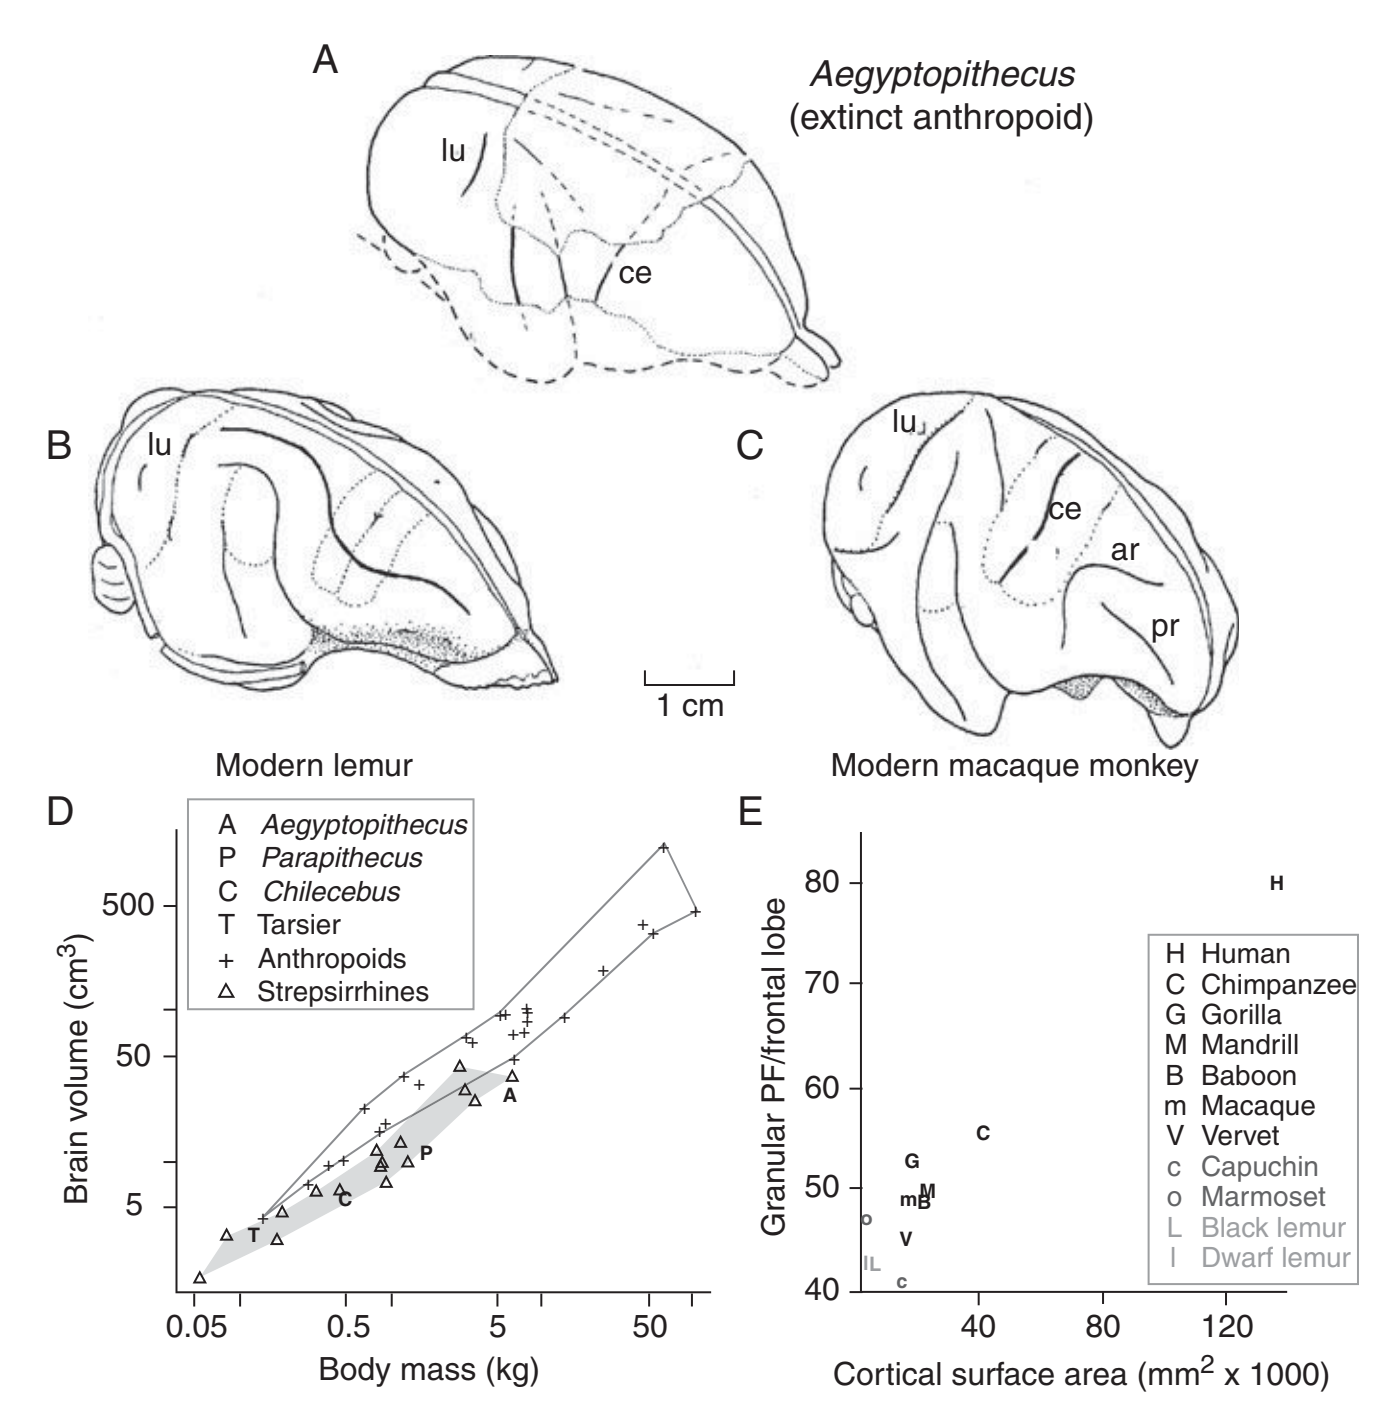
\includegraphics[width=0.8\linewidth]{image_pfc/Fig_2_7}
	\caption*{图2.7(A-C)是已灭绝的人猿类动物埃及长颈猿的化石内脑凸与现代的原猴(B)和恒河猴(C)进行比较。正前方朝右,背部向上。缩写:ar,弓形沟; ce,中央沟; lu,月状沟; pr,主沟。图(B)和(C)中的虚线指示自尾到头的大致位置:主要视觉、主要听觉、主要体感和主要运动区域。 (D)所选已灭绝和现代灵长类动物的脑大小与体大小之比。缩写:A,埃及长颈猿; C,智利狨; P,帕拉猴; T,狐猴。 (E)额叶小叶颗粒前额皮层占前额皮层(表面积)比例随皮层大小变化的百分比。 (A-C)转载自Radinsky L. 1975. Primate brain evolution. American Scientist 63:656–63。 (D)修改自Bush EC、Simons EL、Allman JM.高分辨率计算机断层扫描研究化石人猿帕拉猴头骨:对灵长类动物感觉系统演化历史的新见解。解剖学记录:综合解剖学和进化生物学的进展281a: 1083-7,2004,John Wiley and Sons,获得许可。 (E)修改自Elston GN、Benavides-Piccione R、Elston A、Zietsch B、Defelipe J、Manger P、Casagrande V、Kaas JH。灵长类动物颗粒前额皮层的特化:对认知加工的影响。解剖学记录:综合解剖学和进化生物学的进展288a:26-35,2006,John Wiley and Sons,获得许可。}
\end{figure}

图2.7D还绘制了另一种灭绝的类人猿副猿(Bush等人,2004),这种类人猿接近最早的类人猿(Simons,2004)。与埃及古猿一样,副猿(图2.7D中的点P)的大脑处于灵长类身体大小的范围内,早期新大陆猴智利猴(图2.7D中的点C)(Sears等人,2008)和Homunculus(Kay等人,2006)也是如此。

根据图2.7D中的点T,著名的灵长目动物夜猴的大脑也属于半猴类的范畴,这进一步证明了较小的“原猴”级别和较大的“类人猿”级别之间的区别。早期旧大陆猴和新大陆猴的大脑大小在化石证据中显示出独立演化的趋势,考虑到它们相对较小的大脑,早期猫猴和早期扁鼻猴表明大脑的扩展独立进行。因此,类人猿的大脑可能一直保持在半猴类的水平,直到大约在3400万年前扁鼻猴和猫猴分裂之后。

在本书的其余部分,我们将仅仅为了区分较大的后代物种与早期的、大脑较小的类人猿,将已经达到这种大脑上升档次的物种称为先进类人猿。需要注意的是,在生物学中,先进一词仅仅意味着相对于祖先状态的某些分化,而原始一词仅仅意味着与祖先状态的密切相似。这些术语并不涉及相对能力或复杂性。此外,由于我们对类人猿PF皮层的大部分了解来自于猕猴和人类这些猴类动物的研究,因此我们归因于先进类人猿的某些特征可能代表猕猴的专门化。

根据Radinsky(1975)的研究,视觉皮层的扩展已经达到了现代类人猿的范围,而埃及古猿的大脑处于鼻猴大小范围内。因此,相对较近的额叶扩张似乎是现代类人猿大脑增长的最大因素。而且,像大脑总体扩张一样,这种额叶扩张似乎在旧大陆和新大陆猴类中独立发生(Williams等人,2010)。因此,比例过大的额叶扩张可能产生了类人猿灵长类动物特征的大脑。

化石内窥镜无法区分颗粒和无颗粒前额皮层,但现代灵长类动物的细胞构造分析可以。Brodmann (1912)测量了现代灵长类动物颗粒前额皮层的大小,表明灵长类动物的大脑越大,新皮质中颗粒前额皮层所占的比例越大。图2.7E显示了几种现存灵长类动物额叶皮质相对于新皮质的大小比例。在代表性的类人猿中,颗粒前额皮层占新皮质的9-11%,占额叶皮质的43-50%(Elston等人,2006)。代表性的原猴则对应的数值为7-8%和41-43%。与颗粒前额皮层不同,颞皮层在大脑变大时并没有成比例地变大(Rilling\&Seligman,2002)。因此,在灵长类动物演化中,颗粒前额皮层似乎比其他大脑皮层部分成比例地扩展。正如前面所解释的,比较解剖学的证据表明这种增加涉及PF皮层内新区域的发展。当然,我们也不能排除类人猿额叶皮层其他部分的扩张。

这个结论表明,前期的人猿类甚至最早的猴形类动物的大脑皮层额叶皮层前区还没有发生扩张。这一结论有一个重要的含义,即导致人猿类起源的选择性压力可能与导致后来人猿类产生新的颗粒状前额皮层区域的压力不同。为了理解这些后来的选择性因素,我们需要更详细地考虑关键的人猿类创新。

\subsection{白天的生活和中央凹}
早期的半猴类动物转向了白天活动并进化出灵长类的中央凹,早期的类人猿遗传了这两个特征。眼睛在早期类人猿中也采用了更前面的定位,并且在眼睛后方发展出一个眶骨作为下颌肌肉和眼睛之间的隔墙。

早期人猿类动物向日行性生活的转变以及灵长目中的“中央凹”的进化,为人猿类动物的日间行为提供了支持。相对于大眼睛而言,小眼睛需要的光线更少,而所有早期人猿类动物的头骨都有相对较小的眶窝,这是白天生活的一个强烈指示(费格尔1999)。比较证据表明,几乎所有现代人猿类动物都有白天活动的模式,但很少有其他灵长类动物有这种模式(Heesy\&Ross 2004)。早期人猿类动物继承了日行性生活,并且大多数仍然保留了这一特征。

凸眼动物视网膜窝的起源证据完全依赖于比较证据。夜眼猴和类人猿的视网膜窝都具有许多共同特征。视网膜窝直径约为0.7毫米,每平方毫米约有25万个锥形光感受器。它位于更大的视网膜特化区域——黄斑区内。在所有凸眼动物中,视网膜窝缺乏血管、杆状光感受器和视网膜神经节细胞。即使在视网膜窝内,光感受器的密度也存在陡峭的梯度,最高的锥形密度位于其中心位置。相比之下,夜眼猴的中央视网膜由微小的杆状光感受器主导。

许多脊椎动物独立地进化出了具有凹点的视网膜,如在鱼类中可能有三次,爬行动物中也可能有三次,在早期鸟类中也有单独的进化事件,而在灵长类进化史上则有一次(Ross,2004)。与其他哺乳动物相比,灵长类的凹点是独特的,这意味着其他的(半猴类)灵长类也缺乏凹点。一些哺乳动物(如食肉动物,包括猫和狗)进化出了类似于半猴类凹点的视网膜特化结构。例如,猫具有视网膜中心附近的一条视线,由许多广泛、水平排列的光感受器组成。这条视线缺乏高密度的圆锥感受器和大部分其他的半猴类凹点的定义特征(Hughes,1977)。这条视线几乎肯定是独立进化的。

类人猿眼睛更前置的定位突出了早期灵长类进化的一个特征。随着视点中央的锐度和立体视觉的进化,增强了视觉领域的重要性。正如前面提到的,眼睛的前置定位程度与大脑大小和视觉皮层大小相关(Barton 1998),而视觉皮层的大小与视觉区域数量的增加有关(Kaas 2006)。它还与处理高锐度视觉的视觉处理通道的大小相关(Barton 2004)。与灵长类一般一样,这些类人猿的进步使得物体的视觉引导和操作得到了改善。

在人猿进化的后期,旧大陆猴类进化出了人类继承的常规三色视觉。正如先前提到的,这种颜色视觉被称为常规三色性,以区别于许多新大陆猴类中出现的不同的多态性三色视觉,尽管新大陆猴类中的一组豚猴(Alouatta)独立地进化出了常规三色视觉。

色觉感知取决于来自调谐于特定光波长的圆锥形光感受器发出的信号之间的对比。这种对比机制被称为颜色对立。大多数哺乳动物,包括长鼻类灵长类动物,只有两种圆锥体感受器:一种最适应短波长光,另一种最适应长波长光。在猴形类灵长类动物中,长波长类型圆锥体感受器的基因发生了重复和多样化,形成了两种圆锥体,其峰值敏感度略有不同。因此,与祖先的二色性状态相比,猴形类灵长类动物的色觉有了一个额外的维度。在新大陆猕猴中,只有雌性有三种圆锥体,这是通过不同而独立进化的过程实现的。它们使用基因多态性来实现三色性,而不是使用两个不同的基因。

改善的视力、更好的深度感知和改善的色彩视觉为日间觅食提供了明显的优势。事实上,即使没有中央凹,白天在明亮的光线下觅食也会带来觅食和交流的改善。即使没有三色视觉,中央凹也为类人猿提供了一个复杂的、有深度的物体视图。

一种类人猿的日常生活说明了中央凹的重要性。Struhsaker(1980)对一种猕猴红尾猴进行了野外研究。他发现它们每天有21%的时间扫视他们的视觉世界,可能是为了寻找水果、昆虫和捕食者。它们另外花费了17%的时间从一个地方走到另一个地方获取资源,基于它们看到的。一旦到达有丰富食物的地方,它们花费34%的时间进食。总的来说,这些猕猴花费超过70%的活跃时间在观察周围环境和采取相应行动。剩下的时间,这些猕猴花费10%的时间休息,5%的时间进行社交互动,如梳理。比例会因物种而异,但红尾猴似乎足够代表性,可以说明一个观点:随着获得更好的远距离信息的新机制,类人猿会经常环顾四周。

然而,仅仅拥有一个中央凹、改进的深度感知和日间生活,很可能不足以促进在进化先进的类人猿中出现新的PF颗粒区。大部分视觉发展都发生在这些动物的额叶扩展之前。正如之前所解释的,前额叶扩张发生在猴形目和新大陆猴之间的分裂之后,但中央凹和更向前定位的眼睛出现在类人形目的早期。改进的视力和日间觅食并没有直接推动额叶的扩张,而是推动了视觉皮层的明显变化,包括其扩张和许多新的视觉区域的出现(Kaas 2006, 2012)。后来,对于狭鼻猿来说,例行的三色视觉的发展强化了这些发展。

在人猿的视觉专门化中,只有三色视觉是最近出现的,可以解释人猿大脑和PF皮层的扩张。正如我们刚才提到的,常规的三色视觉最早出现在早期类人猿中。我们不能排除三色视觉作为驱动PF皮层扩张的推动力,但我们怀疑它。PF皮层的扩张需要放在整个皮层扩张的背景下,新的PF区域与其他新的或扩大的区域一起发挥其作用。

例如,Rathelot和Strick(2009)发现,初级运动皮层(区域4)的尾部部分具有直接单突触投射到脊髓运动神经元的大部分神经元,Kaas(2004)得出结论,初级运动皮层的出现可能发生在人猿类动物中。尾部区域在人猿类动物中似乎是一个新的区域,就像前面解释的那样。因为它接收皮肤输入(Strick\&Preston 1978;Tanji\&Wise 1981),我们认为它可能在物体操作中发挥作用。重要的是,这种能力在水果选择中可能特别重要。一种特殊的皮肤感受器称为梅氏小体,集中在指尖和其他无毛表面的表皮脊线中。这些高度敏感的感受器通过快速适应的响应对皮肤变形做出反应,这意味着它们信号皮肤表面施加的小力和这些力的变化。对九种人猿类动物物种的比较表明,梅氏小体的密度与其水果消费量的程度相关。这种关系可能反映了使用硬度和软度评估水果成熟度的能力的变异,这是通过触诊和操作探测的(Hoffmann等人,2004)。初级运动皮层的皮肤输入与三色视觉关系不大,但在某些方面可以理解为发挥类似的作用。人猿类动物手部集中的触觉感受器因此被称为触觉“黄斑区”。

因此,PF皮层的扩张和新的PF区域的增加应该被视为更普遍的大脑扩张的一部分,其中许多脑区都出现了新的或扩张的区域。三色视觉、高分辨率的中央凹视觉和增强的深度知觉使人猿能够利用日间生活的好处进行觅食和交流;但它们本身似乎不足以解释在PF皮层内出现大量新区域的原因。在高级人猿中,某些不只是视觉的东西驱动了额叶的扩张。

高分辨率、三色视觉一旦进化,就需要专家才能区分所有可能的细微差别,而这种专业技能来自感知学习。猕猴在试图进行这种区分时,随着经验的增加,对非常相似颜色之间的微小差别变得非常娴熟(Gaffan 1996)。因此,额叶颞下皮层的扩展在一定程度上反映了对颜色、视觉纹理等方面进行细微差别判别的需求。对于猕猴来说,颞下皮层的损伤会导致严重的色调差异检测障碍,尤其是对于非常相似的色调(Huxlin 等人 2000)。同样地,额叶颞下皮层的扩展也反映了对高分辨率中心视觉的需求。颞下皮层的损伤会导致高度局部化的中心视觉障碍,而不是针对更大视野的判别(Horel 1994)。正如第7章所解释的那样,这些颞下皮层区域是颗粒PF皮层的重要输入来源。

为了帮助我们理解导致人猿PF皮层内出现新区域的选择压力,我们需要关注白天生活的成本,而不是它的好处。正如前面所解释的那样,白天觅食可以提高使用远距离视觉线索来检测和评估资源、识别潜在捕食者和进行社交交流的能力。然而,这些好处也伴随着几个成本:增加的被捕食的风险、更激烈的竞争和热应激。

在白天觅食使得动物更容易受到捕食的威胁,因此类人猿需要在觅食期间和间歇期间寻找捕食者。视网膜上的凹点的发展有助于检测捕食者,但是相较于它们的夜行祖先,风险仍然更大。

白天活动还会增加与其他白天活动的动物的食物竞争,其中一些最初可能更适应于白天生活。人猿类动物与果蝠、松鼠、食果鸟以及一些有袋类动物竞争,这也包括了一些地方的情况(Oates 1987)。毕竟,鸟类可以直接飞到它们的食物上,而灵长类动物却不能。同一社交群体的成员也会带来额外的竞争,所有形式的竞争在短缺期间变得更加重要。正如前面提到的,这种竞争是因为白天活动的物种通常比夜间活动的物种有更大的社交群体,这可能是为了防止被捕食者袭击。

白天觅食也增加了对热应激的敏感性,这是夜间觅食者所避免的问题。在大多数灵长类动物生活的热带地区,下午气温通常会升至30-35°C或更高,而随着热负荷的增加,调节内部温度的能力开始恶化。在相当长的时间内,热带的高温使觅食变得危险,大多数人类类动物在早晨醒来后和夜间休息前觅食(Oates 1987)。因此,即使在热带的长而规律的白天,热应激也限制了觅食的时间。

时间限制必定加剧了食物资源的竞争,而被掠食的风险也让所有觅食选择变得更加复杂。我们认为,这些问题选择了改善觅食选择并迅速学习如何做到这一点的能力。在第8章中,我们认为,进化更古老的试错学习机制产生了太多的不良选择,而皮层颗粒质前额叶的新部分实现了一种改善觅食选择的学习机制。因此,高级的类人猿可以比它们的祖先更有效地竞争稀缺资源。

理解新的颗粒PF皮层如何提供这种优势,我们需要知道先进的类人猿如何觅食,为什么关键资源有时会变得稀缺,以及为什么糟糕的觅食选择会付出如此高昂的代价。

\subsection{体型、饮食和类人猿的移动方式}
与其他动物一样,类人猿需要寻找和消耗能量丰富的食物,包括蛋白质及其氨基酸、各种矿物质、维生素、液体和其他营养素,如特定的脂肪酸。作为一个群体,现代类人猿通过吃水果、叶子、昆虫、花朵、根、树皮、种子和坚果以及树胶等多种食物来满足这些需求。大多数类人猿可以被归类为杂食动物。尽管存在这种饮食多样性,它们可以被分类为食虫动物(主要是昆虫食),果食动物(吃水果的动物)、叶食动物或者这些类别的某种组合。

体型对饮食选择有很大的制约作用,而人猿的体型在其进化过程中发生了巨大的变化。最早出现的人猿,出现在相对早期的灵长目历史上(约 5500 万年前),体重不到 100 克。他们的体型和牙齿结构的化石证据支持了这样一个观点,即早期的人猿主要以水果和昆虫为食(Fleagle 1999;Rose 2006),也许在这方面与栖息在细枝上的其他生物并没有太大的不同。

后来的类人猿体型变得更大,现代大部分类人猿重量超过1公斤。直到约3400万年前的大平鼻亚目-狭鼻亚目分裂后,化石类人猿体型没有发生明显的增加 (Williams等人,2010)。例如,在本章早些时候提到的化石类人猿埃及古猿和副猿比最早的类人猿大得多,体重为2-4千克。一旦出现更大的类人猿物种,它们就会适应牙齿形态的变化,这表明它们的饮食主要由水果 (Williams等人,2010)和嫩叶 (Kirk\&Simons,2001; Dominy,2004) 组成。

随着体型的增大和饮食方式的变化,大脑额叶的扩展和脑大小的上升逐渐发生,这些变化在本章前面已经讨论过。随着这些动物体型的增大,它们需要更多的能量。因此,随着人猿的体型变大,它们不得不以与祖先不同的方式利用资源。

因此,它们放弃了早期灵长类使用的跳跃和抓握式的运动方式,成为树栖四足动物:它们使用四肢在更大的树枝间移动。这个结论来自现代人类猿类中这种运动方式的普遍性(Schmidt 2010)以及化石证据(Fleagle 1999)。树上路径对能量有很高的需求(Janson 1988),特别是在移动时高度变化较大的情况下。因此,它们更大的体型和运动方式都需要高能量的摄入。

高级类人猿采用的新的运动方式扩展了它们的觅食范围。即使考虑代谢率等因素,现代高级类人猿的家域范围仍然很大(Martin 1981)。许多高级类人猿仍然是树栖的四足动物,通过耗费大量能量的杂技式运动方式在更大的树枝上移动。几种高级类人猿(包括猕猴)后来发展出了陆地四足动物的运动方式,而一些新大陆猴和大猩猩则进化出了悬挂运动的方式,当然,人类祖先则进化出了直立二足的运动方式。悬挂运动允许更大的动物重新进入细枝分支生态位。与树栖四足动物相比,陆地四足动物节省了一些能量成本(Janson 1988),但仍然很昂贵。直立二足步态有许多后果,其中包括失去了最早的灵长类动物进化出的许多后肢抓握专业化特征,如食果猴。

总之,迄今为止我们的讨论可以总结为:随着类人猿在大约3400万年后变得更大,它们的觅食范围扩大,并且从成熟的水果和嫩叶中获得了大部分的营养。这些食物在获取所需能量方面成本高,并且涉及相对较高的被捕食风险。请回想一下,表征先进类人猿的大脑扩张也发生在大约3400万年前,也就是新大陆和旧大陆类人猿分化的时间。

理解这些动物所面临的风险和成本的性质和强度,以及这些因素如何可能导致新的颗粒状前额皮质区域,我们需要探讨人猿猴面临的觅食问题。

\subsection{类人猿的觅食方式}
大多数现代人猿强烈依赖于利用被被被子植物树木产生的资源,主要是水果和叶子。对于许多灵长类动物来说,昆虫也是重要的蛋白质和氨基酸来源,但它们的生物量和密度很少与被子植物树木和其他植物提供的资源相匹配。

随着先进类人猿开始依赖产自被子植物树木的高能量产品,它们面临了一个问题。这些资源的分布呈现出一片片点状,分散在它们的栖息地范围内。因此,它们的饮食需要更多的觅食和休息更少的时间。正如我们所见,热应激和被捕食的威胁使得热带白天觅食者在获取食物方面时间有限。考虑到竞争的激烈程度和其运动方式的成本高昂,这些相对较大的类人猿必须做出良好的觅食选择。

人猿的觅食策略在很大程度上是决定要访问哪些树木。任何一种树木品种的树木都分散在一个给定的人猿物种的活动范围内。每种树木都有其特定的结果模式,通常涉及结果时间间隔的不一致性和一年中的戏剧性变化(Chapman等人,1999; Janmaat等,2006)。同样的概念也适用于树叶。在给定的栖息地中,非毒性的可食用叶子植物种类很少,而树木会以高度季节性的方式产生这些叶子(Dominy,2004)。只有幼嫩的叶子提供高蛋白质相对于纤维素的营养价值。鉴于大多数人猿无法在热带地区食用或消化大量植物物质,这些变化会导致频繁和不可预测的食物短缺。我们提出,这种资源的波动性提供了促进人猿前额皮层中新区域进化的推动力之一。

据Zuberbühler和Janmaat (2010)指出,大型猕猴的活动范围包括约100,000棵树,其中不超过4%的树在任何一个时间都有成熟的果实。Janmaat等人 (2006)估计,对于灰颊芒巴(Cercocebus)来说,一些群体的活动范围可能只有50棵树结果,而它们通过它们的领土。尽管它们的热带环境中有数千棵树,但人猿猴通常只在任何给定时间内的少数树种上觅食,重点关注具有高密度树和每棵树上有高密度果实的树种 (Janson 1988; Eckhardt \& Zuberbühler 2004)。这种觅食策略使它们容易受到这些树种产量不足的影响,而相同的概念也适用于营养丰富的树叶的产量。

进一步复杂化问题的是,不同树种成熟果实或嫩叶的比例在树种之间,甚至在同一树种不同年份和不同地区也存在显著差异。在一项野外研究中,一种特定的树种在12年中只结果了四次,有时在 5\% 的树上结果,在其他时候在 50\% 的树上结果。在某个领域内的一个站点中,一个给定树种的60\%树上有果实,但在其他站点相同种类的树上则完全没有果实(Chapman等人,2004年)。

这些统计数据提供了人科动物所面临的巨大问题的一瞥。加上在高温下有限的觅食时间、被捕食风险以及来自其他动物的竞争,受欢迎的树木生产的不一致必须会导致周期性的营养危机。增强克服这些匮乏时期的能力,同时减少被捕食的风险,将有助于促进适应度的提高。

我们强调这种增强能力是在人猿类的进化历史上的某个特定时间和地点发展起来的。我们不知道这些变化确切发生的时间和地点,但它们可能发生在大约 3400 万年前的热带地区。例如,气候冷却大约在 3500 万年前发生,导致可用资源普遍不足。因此,人猿类需要多样化其饮食习惯以利用后备资源。根据多米尼(2004)的观点,这时食叶变得更加频繁(Kirk \& Simons 2001),而三色视觉可能已经进化出来以区分年轻、有营养的叶子和老叶。正如我们所看到的,人猿类的大脑扩展始于大约同一时间,其中许多扩展涉及颗粒状前额皮质。

许多体型较大的动物需要解决资源波动的问题,但我们认为,人形类动物以不同的方式解决了这个问题,这种解决方式依赖于它们的颞叶后枕皮层。在本章早些时候,我们回顾了证据表明随着人形类动物的身体、大脑和额叶变得更大,新的颞叶后枕皮层区域出现了。我们提出这些新区域让人形类动物能够克服断断续续的食物短缺、激烈的竞争和捕食风险所带来的问题。这个提议并不意味着其他动物群体缺乏克服类似问题的能力。在它们分化之后,每个谱系都会面对自己的问题和机遇,因此平行进化是普遍存在的。

野外观察已经确定了一些寻食策略的特征,它们构成了解决资源波动问题的人猿方式:\par
1.树木的估价。猕猴根据对个体树木的估价做出采食选择,其中包括对于除最有经验的类人猿外看起来相同的物种(Zuberbühler \& Janmaat 2010) 。类人猿根据先前接触过该树木果实和叶子的经验来评估单个树木,这得到了猕猴之前在该树上吃过高质量水果的证据支持(Janmaat et al. 2006);\par
2.适应性在食物短缺期间。在食物短缺期间,以水果和昆虫为食的人类猿倾向于增加觅食时间,减少休息时间,并增加彼此之间的竞争(Kavanagh 1978; Oates 1987)。相比之下,食叶者则倾向于节约能量并减少觅食。在这种情况下,以水果为食的人类猿也表现出显著的灵活性,不太受欢迎的食物成为回退食品的目标。例如,Kavanagh(1978)研究了干季果实减少的两个地点的绿猴,其中一个地点的绿猴群体通过增加觅食时间并减少饮食多样性,集中于吃昆虫而不是水果来应对干季果实减少的挑战。另一个绿猴群体通过减少觅食时间并增加饮食多样性来应对相同的挑战,从以水果为主导的饮食转变为将花和昆虫组合在一起的回退饮食。这两个群体之间的差异表明,适应性——采用替代觅食策略的能力——使人类猿能够克服优选食物不规则短缺的问题;\par
3.使用提示和标志。人猿的觅食选择可以依赖与食物相关的声音和视觉提示。这些标志包括其他灵长类动物和争夺同一资源的鸟类竞争者发出的声音。Janmaat等人(2006年)研究了野生猴的行为,当它们遇到新出现或成熟的水果时,这些猕猴会注意到周围有已经被嘈杂的黑猩猩或犀鸟占据的树,这两种都是热衷于水果的强有力的果食动物,尽管存在被黑猩猩捕食的风险,但猕猴还是更快地接近这些树;\par
4.基于同步性预测食物生产。猕猴还利用在一棵树上发现食物的信息,预测其他相同种类的树上也有可用的食物。Menzel(1991年)研究了野生的日本猕猴,发现在它们的家园范围内放置成熟的柿子会诱使它们访问柿子树,即使野生树木没有任何成熟的果实。猕猴必须知道柿子树的位置,并且已经学会根据类似树上的果实来预测果实的成熟;\par
5.猕猴似乎会监测并记住树木以前的食物产量历史来预测未来的食物可用性(Milton 1988)。即使没有感官线索指导,它们向有果树移动的速度也比向无果树移动的速度快得多。它们甚至更快地向果实数量更多的树移动(Zuberbühler\&Janmaat 2010);\par
6.热量可以促进植物新陈代谢以及食物的生产,也会加速水果的成熟。猕猴利用最近的天气条件来做出觅食选择,当天气更热时,它们会更快地返回到之前产生过丰富食物的树上(Janmaat等人,2006)。

\subsection{小结}
现场研究表明,人猿类灵长动物面临严重的资源波动、被捕食的危险,以及时间限制和资源竞争。在这些条件下,适应食物短缺期间的策略转换、使用远程食物可用的迹象以及使用树木生产历史的记忆来预测食物出现的位置等方法都是有益的。

我们认为,新的细颗粒前额区使人猿能够以他们特有的方式适应零星的食物短缺问题。\par
$\bullet$第3章的论述表明,极端前额叶皮层使人类类群能够学习在特定情境下做出哪种觅食选择,即使过去只做过一次这个选择。\par
$\bullet$第6章认为,背侧顶叶皮层有助于根据视觉事件的顺序或时间经过来做出采食选择,并规划目标序列以提高采食效率。\par
$\bullet$第7章认为,腹侧前额皮质是视觉和听觉信号指导采食选择的基础,包括通过中央凹、三色视觉检测到的近距离和远距离的食物可用信号。\par
$\bullet$第8章的论述表明,新的颗粒状区域共同发挥作用,使得人猿能够通过快速学习和使用抽象规则和策略来适应新情况,从而利用单个事件来选择觅食目标。

所有这些能力有助于进行更好的觅食选择,我们提出新的颗粒状前额皮质区在进化过程中为灵长类动物提供了这些优势,使其胜过祖先。

\section{总结}
\begin{figure}[!htb]
	\centering
	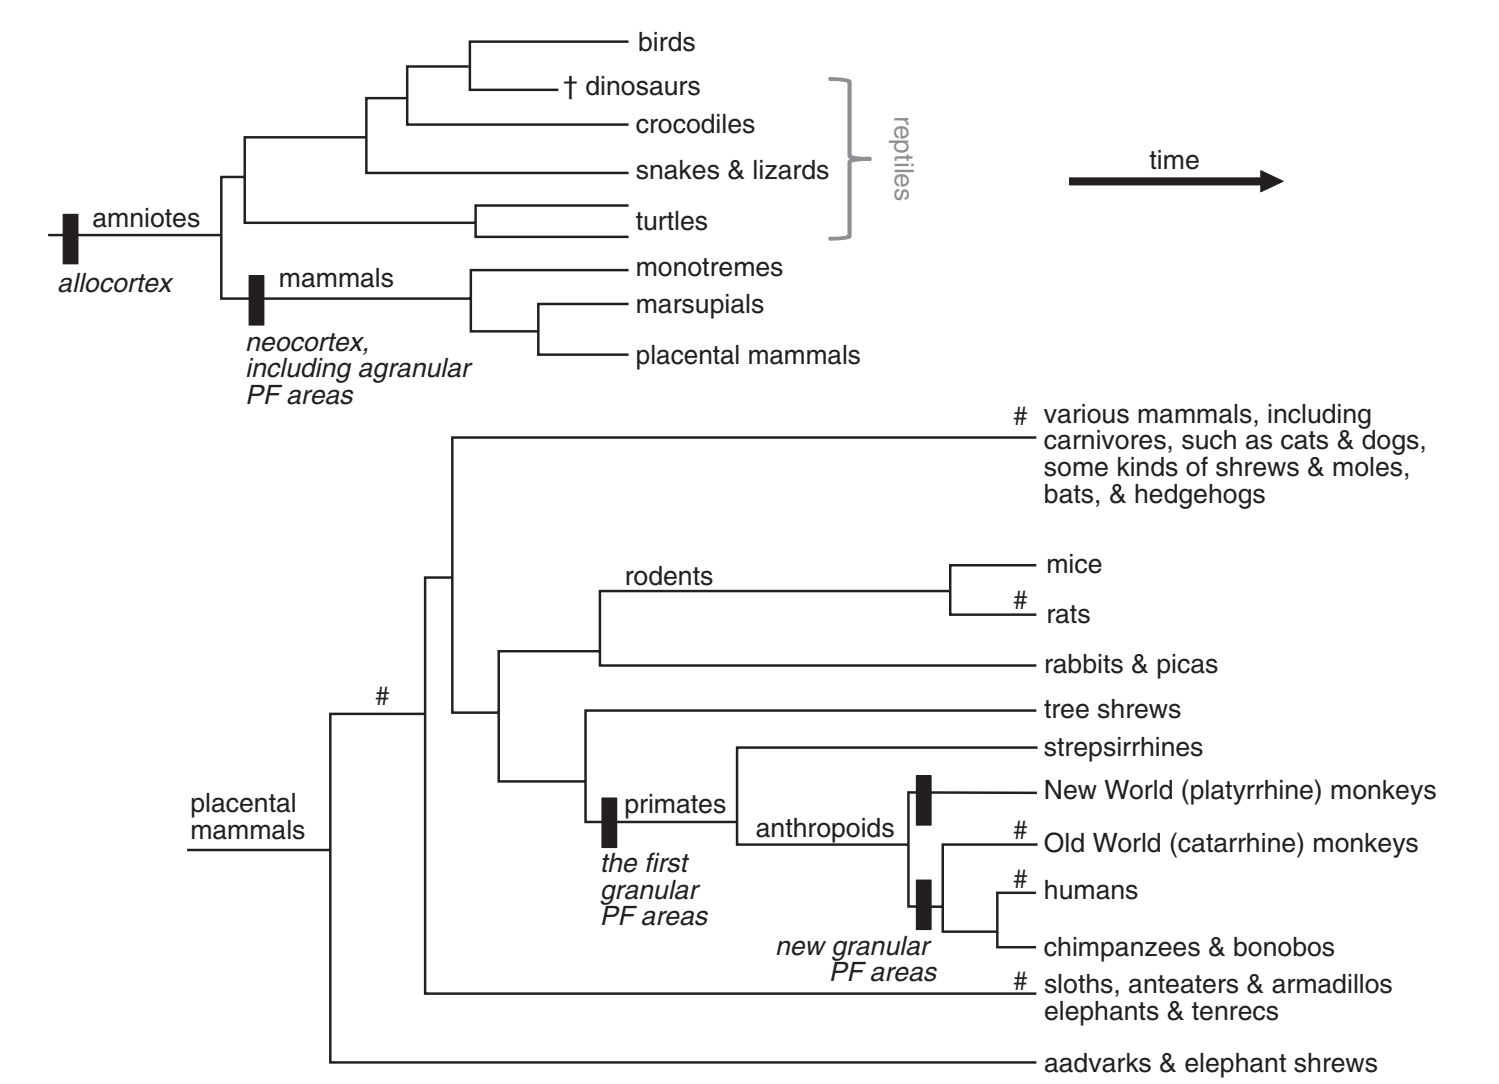
\includegraphics[width=0.8\linewidth]{image_pfc/Fig_2_8}
	\caption*{图2.8 上图:爬行动物、哺乳动物和鸟类的选定群体之间的进化关系。 下图:选定有胎盘的哺乳动物之间的进化关系。格式与图2.5相同。符号(\#)表示深度分支谱系,这些谱系可以作为比较行为研究的可靠基础,以及它们的共同祖先。图中内容摘自Murray EA、Wise SP、Rhodes SE所著《The Neurobiology of Sensation and Reward》(2011),由Taylor and Francis出版社授权使用。}
\end{figure}
PF皮质的进化是分阶段进行的,图2.8有助于对它们进行梳理。一个阶段发生在早期哺乳动物身上,产生了PF皮质的非颗粒部分。早期哺乳动物利用夜间觅食的生态位,新皮质在这些动物中进化出来。非颗粒PF区域与新的视觉、听觉和体感区域一起,支持了这个新生态位中的觅食选择。第3章和第4章讨论了非颗粒PF区域,表4.1提出了一些关于它们在觅食选择中具体贡献的想法。

在PF皮层的后期演化中,颗粒PF皮层出现在早期灵长类动物身上,当它们适应了生活在树的细小树枝上的生活时,它们可以利用嫩叶、水果、花朵、花蜜和昆虫。第一个颗粒PF区域包括尾部PF皮层和眶上皮质的颗粒部分的同源物。这些新的颗粒PF区域当时和现在都在搜索食物和食物迹象方面发挥作用,并根据当前的生物需求评估它们的价值。第4章和第5章涉及这些主题。

在PF皮层的演化的最后一个阶段发生在人猿的进化过程中。早期的人猿从其狭鼻亚目的祖先那里继承了白天觅食和中央凹,而后来的人猿发展出了三色视觉。随着人猿变得更大,它们在更大的家域内觅食,并依赖于特定树木的食品。因此,它们变得容易受到这些食物的短缺的影响。比较的证据表明,此时出现了几个新的PF领域:背侧PF皮质,腹侧PF皮质,以及可能还包括极端PF皮质。我们提出,这些新的PF领域在食物短缺和激烈竞争时提供了适应性优势。在第3-8章中,我们认为这些皮层区域通过减少增加捕食风险、浪费精力或产生比其他选择更少好处的选择的频率,提高了觅食的效率。

在实验室中,浪费努力或产生较少效益的选择被称为错误。错误的明确定义以及实验室行为和自然觅食之间的巨大差异几乎不需要提及。例如,在野外,觅食选择经常涉及哪棵树或哪个位置接近以获取食物,而在实验室中,对刺激的反应通常涉及到伸手或眼部运动以获得奖励。觅食通常涉及物体(包括食物)的操作,但只有少数实验室测试探索了像物体操作这样复杂的动作。实验室测试有试验,但是觅食选择很少适合这样简单的时间划分。觅食还经常涉及社交互动,实验室研究只有在最近才开始认真研究这个领域。

虽然如此,实验室实验为猕猴提供了在地点和物体之间做出选择的机会,并且这些选择会产生它们需要和消耗的食物或液体。因此,实验室研究可以探索有助于成功觅食的认知能力。

Hayden等人(2011年)的一项开创性研究试图模拟人猿在从开发减少的资源转而探索更遥远的资源时所做的种类狩猎选择。第3章阐述了这个实验的结果,但我们在这里提到它是因为这个任务是一个使用简单的彩色形状、变量延迟期和注视性眼动来研究人猿所做选择的例子,这些选择包括对视觉信号的反应,估计到达远程资源所需的时间以及使用四足步态行走。

因此,尽管野外觅食和控制实验室实验之间存在明显的差异,但许多有益于野外觅食的认知能力可以在实验室中进行研究。

1.采食类灵长类动物需要将其行为与所获得的资源结果联系起来,某些实验任务可评估猕猴如何学习这种联系。第三章回顾了一些研究,例如探讨了猕猴如何学习采取哪些行动以最小的努力获得最多的资源;\par
2.寻找食物的灵长类动物还需要将寻找目标(如物品)与食物结果联系起来。它们不仅需要学习食物或液体的一般价值,还需要根据当前的需求来评估这些资源。第四章回顾了一些任务,其中猕猴需要在一些与一定数量或概率的食物或液体相关联的物品之间进行选择。其他实验可以改变反映当前生物需求的动机因素,例如允许猕猴食用某种食物以达到饱食的状态;\par
3.在自然觅食中,动物同时看到许多刺激,并将其中许多记忆。他们需要在所有这些杂乱中找到觅食目标,并将注意力集中在它们上面,同时规划达成目标最有效的方式。第5章讨论了评估注意力和搜索能力的实验任务,例如在一片绿色的正方形中挑出一个红色正方形;\par
4.灵长类动物受益于以有序和高效的方式觅食,第6章讨论了许多用于研究行为在时间和空间上的顺序的任务,例如学习通过视觉迷宫导航的光标或在25个不透明门中选择以获取每个门后面的单个花生。觅食还涉及将目标保留在记忆中,这个概念被称为前瞻编码。可以使用成对联想学习任务来研究此功能,其中一个刺激表示另一个刺激应该作为目标;\par
5.当猕猴们环顾四周时,会看到一些资源的标志。第7章讨论了条件视觉运动任务,这些任务研究标志到动作的映射。同样的任务也可以用来研究猕猴如何使用抽象的策略。在野外,这种能力使得类人猿能够将他们对于一般采食的学习迁移到新颖或罕见的采食问题中;\par
6.在资源不稳定的情况下,从单次经历中学习并因此限制无效或有风险的选择是很有益的。在实验室中,这种能力导致快速学习和其他减少错误的机制。第3和第8章回顾了探索这些功能的任务,例如选择嵌入在背景场景中的物体。

第1章阐述了将PF皮层作为一个整体进行解释的目的。但正如本章所示,整体随着时间的推移而改变。早期灵长类动物发展出的PF皮层缺乏现代人类类动物具有的许多颗粒PF区域;早期哺乳动物进化出的PF皮层则缺乏灵长类动物所有颗粒区域。因此,要完全理解PF皮层,我们需要理解部分和整体。为此,我们需要拆开PF皮层。第3章从内侧PF皮层开始。